% JUNA grant-body slide deck
% Compile with: pdflatex juna_grant_body_slides.tex
\documentclass[aspectratio=169,10pt]{beamer}

\usepackage[T1]{fontenc}
\usepackage{amsmath,amssymb}
\usepackage{booktabs}
\usepackage{graphicx}
\usepackage{tikz}
\usepackage{xcolor}
\usetikzlibrary{arrows.meta,positioning,calc,fit,shapes.geometric,decorations.pathmorphing}

\definecolor{bg}{HTML}{F7F3EA}
\definecolor{panel}{HTML}{FFFCF5}
\definecolor{text}{HTML}{1D2528}
\definecolor{muted}{HTML}{657074}
\definecolor{juna}{HTML}{23684A}
\definecolor{rpc}{HTML}{A43B36}
\definecolor{pilot}{HTML}{2D6CDF}
\definecolor{data}{HTML}{6E7378}
\definecolor{nullc}{HTML}{ECE5D8}
\definecolor{gold}{HTML}{C08A2D}
\definecolor{grid}{HTML}{CFC7B7}
\definecolor{accent}{HTML}{0F4C81}

\usefonttheme{professionalfonts}
\setbeamercolor{background canvas}{bg=bg}
\setbeamercolor{normal text}{fg=text}
\setbeamercolor{frametitle}{fg=text,bg=bg}
\setbeamercolor{structure}{fg=juna}
\setbeamercolor{calloutbox}{fg=text,bg=panel}
\setbeamertemplate{navigation symbols}{}
\setbeamertemplate{itemize item}{\raise0.15ex\hbox{\scriptsize$\blacktriangleright$}}
\setbeamerfont{frametitle}{series=\bfseries,size=\Large}
\setbeamertemplate{frametitle}{%
  \vspace{0.25em}
  \insertframetitle\par
  \vspace{0.25em}
  {\color{grid}\rule{0.94\paperwidth}{0.5pt}}
}
\setbeamertemplate{footline}{%
  \hfill{\scriptsize\color{muted}JUNA \textendash{} Doppler-resilient underwater OFDM\quad\insertframenumber}\hspace{0.5cm}\vspace{0.25cm}
}

\newcommand{\metric}[2]{\textbf{#1:} #2}
\newcommand{\channelimage}[1]{\includegraphics[width=\linewidth,height=0.40\paperheight,keepaspectratio]{#1}}
\newenvironment{callout}{%
  \begin{beamercolorbox}[wd=\linewidth,sep=4pt,rounded=true]{calloutbox}\scriptsize%
}{%
  \end{beamercolorbox}%
}

\tikzset{
  block/.style={draw=text, fill=panel, rounded corners=2pt, line width=0.55pt,
                align=center, inner sep=5pt, font=\small},
  arrow/.style={-{Stealth[length=2.4mm]}, line width=0.7pt, draw=text},
  callout/.style={draw=grid, fill=panel, rounded corners=2pt, line width=0.45pt,
                  align=left, inner sep=6pt, font=\small},
  tinycell/.style={draw=grid, line width=0.25pt, minimum width=0.33cm,
                   minimum height=0.33cm, inner sep=0pt}
}

\begin{document}

% =====================================================================
% 1. TITLE PAGE WITH ARL LOGO
% =====================================================================
\begin{frame}[plain]
  \vspace{0.25cm}
  \begin{center}
    \includegraphics[height=2.6cm,keepaspectratio]{arllogo.png}\\[0.30cm]
    {\Huge\bfseries\color{accent} JUNA\par}
    \vspace{0.18cm}
    {\Large A joint receiver--decoder for\\
     \textbf{Doppler-resilient underwater communication}\par}
    \vspace{0.55cm}

    % --- decorative spectrum / motion banner ---
    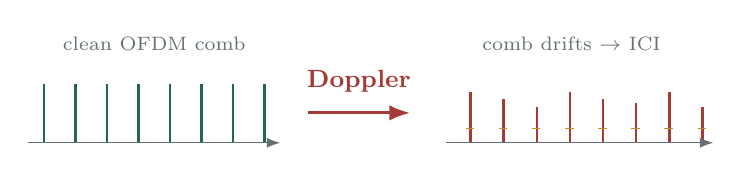
\begin{tikzpicture}[x=1cm,y=1cm,>=Latex]
      % clean comb (left)
      \node[font=\scriptsize,text=muted,anchor=south] at (1.6,1.05) {clean OFDM comb};
      \foreach \x in {0.20,0.60,1.00,1.40,1.80,2.20,2.60,3.00} {
        \draw[draw=juna,line width=1pt] (\x,0) -- (\x,0.75);
      }
      \draw[->,draw=muted] (0.0,0) -- (3.20,0);

      % arrow
      \node[font=\small\bfseries,text=rpc] at (4.2,0.78) {Doppler};
      \draw[->,draw=rpc,line width=1pt] (3.55,0.38) -- (4.85,0.38);

      % shifted + smeared comb (right)
      \node[font=\scriptsize,text=muted,anchor=south] at (6.9,1.05) {comb drifts $\rightarrow$ ICI};
      \foreach \x/\h in {0.32/0.65,0.74/0.55,1.16/0.45,1.58/0.65,2.00/0.55,2.42/0.50,2.84/0.65,3.26/0.45} {
        \draw[draw=rpc,line width=1pt] ({5.30+\x},0) -- ({5.30+\x},\h);
      }
      \foreach \x in {0.32,0.74,1.16,1.58,2.00,2.42,2.84,3.26} {
        \draw[draw=gold,line width=0.4pt,dashed] ({5.30+\x-0.06},0.18) -- ({5.30+\x+0.06},0.18);
      }
      \draw[->,draw=muted] (5.30,0) -- (8.70,0);
    \end{tikzpicture}

    \vspace{0.45cm}
    {\large First milestone review\par}
    \vspace{0.10cm}
    {\color{muted}\small Acoustic Research Laboratory}
  \end{center}
\end{frame}

% 3. PLAIN-LANGUAGE EXPLANATION OF THE PROBLEM (short)
% =====================================================================
\begin{frame}{The problem, in plain terms}
  \vspace{-0.15cm}
  {\footnotesize OFDM sends many \emph{tones} simultaneously \textendash{} each tone carries one BPSK bit ($\pm 1$); $N$ tones $\to$ $N$ coded bits per OFDM symbol.}
  \vspace{0.05cm}

  % --- Compact bit-to-tone mapping diagram ---
  \centering
  \resizebox{0.78\linewidth}{!}{%
  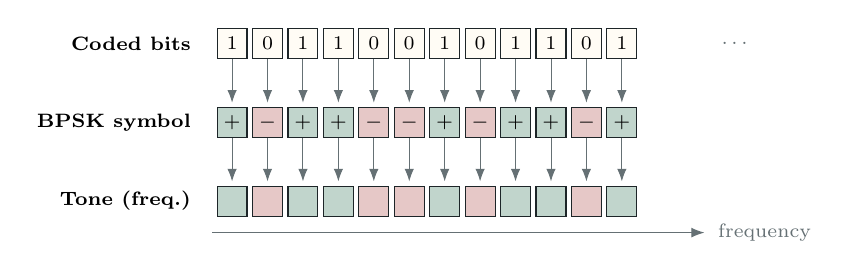
\begin{tikzpicture}[x=1cm,y=1cm,>=Latex,font=\scriptsize]
    \node[font=\scriptsize\bfseries,anchor=east] at (1.0,3.0) {Coded bits};
    \foreach \i/\b in {0/1,1/0,2/1,3/1,4/0,5/0,6/1,7/0,8/1,9/1,10/0,11/1} {
      \pgfmathsetmacro{\xx}{1.4+\i*0.45}
      \node[draw=text,fill=panel,minimum size=0.38cm,inner sep=0pt] at (\xx,3.0) {\b};
    }
    \node[anchor=west,text=muted] at (7.4,3.0) {\,\,\dots};

    \node[font=\scriptsize\bfseries,anchor=east] at (1.0,2.0) {BPSK symbol};
    \foreach \i/\v/\col in {0/$+$/juna,1/$-$/rpc,2/$+$/juna,3/$+$/juna,4/$-$/rpc,5/$-$/rpc,6/$+$/juna,7/$-$/rpc,8/$+$/juna,9/$+$/juna,10/$-$/rpc,11/$+$/juna} {
      \pgfmathsetmacro{\xx}{1.4+\i*0.45}
      \draw[->,draw=muted,line width=0.35pt] (\xx,2.80) -- (\xx,2.25);
      \node[draw=text,fill=\col!28,minimum size=0.38cm,inner sep=0pt] at (\xx,2.0) {\v};
    }

    \node[font=\scriptsize\bfseries,anchor=east] at (1.0,1.0) {Tone (freq.)};
    \foreach \i/\col in {0/juna,1/rpc,2/juna,3/juna,4/rpc,5/rpc,6/juna,7/rpc,8/juna,9/juna,10/rpc,11/juna} {
      \pgfmathsetmacro{\xx}{1.4+\i*0.45}
      \draw[->,draw=muted,line width=0.35pt] (\xx,1.80) -- (\xx,1.25);
      \node[draw=text,fill=\col!28,minimum size=0.38cm,inner sep=0pt] at (\xx,1.0) {};
    }
    \draw[->,draw=muted] (1.15,0.6) -- (7.4,0.6);
    \node[font=\scriptsize,text=muted,anchor=west] at (7.45,0.6) {frequency};
  \end{tikzpicture}}
  \vspace{0.05cm}

  % --- Bottom row: text + waveforms ---
  \begin{columns}[T,onlytextwidth]
    \begin{column}{0.40\textwidth}
      \scriptsize\textbf{Still channel.} Each tone arrives on its own frequency \textendash{} mapping preserved.
      \vspace{0.3em}

      \scriptsize\textbf{Motion / Doppler.} Tones drift off frequency, neighbours overlap, mapping breaks.
    \end{column}
    \begin{column}{0.58\textwidth}
      \resizebox{\linewidth}{!}{%
      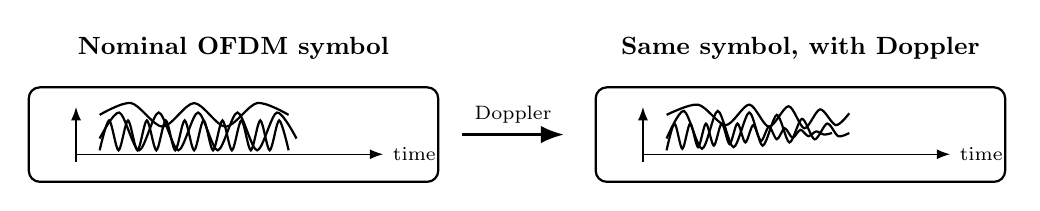
\begin{tikzpicture}[x=1cm,y=1cm,>=Latex]
        \node[font=\small\bfseries] at (3.0,5.8) {Nominal OFDM symbol};
        \draw[rounded corners, thick] (0.4,4.1) rectangle (5.6,5.3);
        \draw[->] (1.0,4.45) -- (4.9,4.45) node[right] {\scriptsize time};
        \draw[->] (1.0,4.35) -- (1.0,5.05);
        \draw[thick] plot[smooth] coordinates {(1.3,4.95) (1.7,5.10) (2.1,4.80) (2.5,5.10) (2.9,4.80) (3.3,5.10) (3.7,4.95)};
        \draw[thick] plot[smooth] coordinates {(1.3,4.65) (1.55,4.98) (1.8,4.50) (2.05,4.98) (2.30,4.50) (2.55,4.98) (2.80,4.50) (3.05,4.98) (3.30,4.50) (3.55,4.98) (3.80,4.65)};
        \draw[thick] plot[smooth] coordinates {(1.3,4.50) (1.42,4.88) (1.54,4.50) (1.66,4.88) (1.78,4.50) (1.90,4.88) (2.02,4.50) (2.14,4.88) (2.26,4.50) (2.38,4.88) (2.50,4.50) (2.62,4.88) (2.74,4.50) (2.86,4.88) (2.98,4.50) (3.10,4.88) (3.22,4.50) (3.34,4.88) (3.46,4.50) (3.58,4.88) (3.70,4.50)};

        \node[font=\small\bfseries] at (10.2,5.8) {Same symbol, with Doppler};
        \draw[rounded corners, thick] (7.6,4.1) rectangle (12.8,5.3);
        \draw[->] (8.2,4.45) -- (12.1,4.45) node[right] {\scriptsize time};
        \draw[->] (8.2,4.35) -- (8.2,5.05);
        \draw[thick] plot[smooth] coordinates {(8.5,4.95) (8.9,5.08) (9.25,4.82) (9.55,5.08) (9.80,4.80) (10.05,5.06) (10.25,4.78) (10.45,5.02) (10.65,4.82) (10.82,4.97)};
        \draw[thick] plot[smooth] coordinates {(8.5,4.65) (8.72,5.00) (8.95,4.52) (9.15,5.00) (9.35,4.54) (9.55,4.98) (9.72,4.56) (9.90,4.95) (10.06,4.60) (10.22,4.90) (10.38,4.64) (10.54,4.84) (10.68,4.68) (10.82,4.72)};
        \draw[thick] plot[smooth] coordinates {(8.5,4.50) (8.60,4.84) (8.70,4.52) (8.80,4.84) (8.90,4.54) (9.00,4.84) (9.10,4.56) (9.20,4.84) (9.30,4.58) (9.40,4.84) (9.50,4.60) (9.60,4.82) (9.70,4.62) (9.80,4.80) (9.90,4.64) (10.00,4.78) (10.10,4.66) (10.20,4.76) (10.30,4.68) (10.40,4.74) (10.50,4.70) (10.60,4.72)};

        \draw[very thick,->] (5.9,4.7) -- (7.2,4.7);
        \node[font=\scriptsize] at (6.55,4.95) {Doppler};
      \end{tikzpicture}}
    \end{column}
  \end{columns}
\end{frame}

% =====================================================================
% 2. ONE-MINUTE PITCH
% =====================================================================
\begin{frame}{Where we are, in one minute}
  \vspace{0.1cm}
  \begin{columns}[T,onlytextwidth]
    \begin{column}{0.32\textwidth}
      \begin{beamercolorbox}[wd=\linewidth,sep=6pt,rounded=true]{calloutbox}
        \textbf{\color{rpc} The problem}\\[0.2em]
        \scriptsize Doppler (motion) breaks subcarrier orthogonality \textendash{} energy leaks between carriers (ICI).
      \end{beamercolorbox}
    \end{column}
    \begin{column}{0.32\textwidth}
      \begin{beamercolorbox}[wd=\linewidth,sep=6pt,rounded=true]{calloutbox}
        \textbf{\color{accent} State of the art}\\[0.2em]
        \scriptsize \textbf{RPC} \textendash{} a recursive partial-FFT combiner \textendash{} corrects the phase/weighting and recovers symbols under Doppler. \emph{Combiner weights are learned from pilots} \textendash{} so it is pilot-hungry.
      \end{beamercolorbox}
    \end{column}
    \begin{column}{0.32\textwidth}
      \begin{beamercolorbox}[wd=\linewidth,sep=6pt,rounded=true]{calloutbox}
        \textbf{\color{juna} What JUNA does}\\[0.2em]
        \scriptsize Combiner weights, soft symbols, and LDPC decoding are trained in a \textbf{single joint learning process} \textendash{} the code shares the load. \textbf{Fewer pilots} at the same reliability \textendash{} so \textbf{higher data rate}.
      \end{beamercolorbox}
    \end{column}
  \end{columns}

  \vspace{0.20cm}
  \begin{center}
  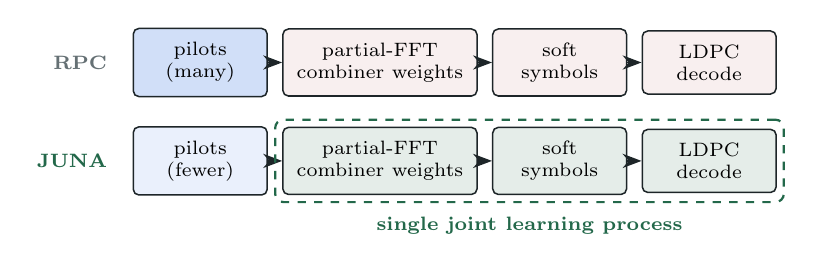
\begin{tikzpicture}[node distance=0.18cm,font=\scriptsize]
    % RPC row
    \node[block,minimum width=1.7cm,minimum height=0.55cm,font=\scriptsize,fill=pilot!22] (rp1) {pilots\\(many)};
    \node[block,minimum width=2.4cm,minimum height=0.55cm,font=\scriptsize,right=of rp1,fill=rpc!8] (rp2) {partial-FFT\\combiner weights};
    \node[block,minimum width=1.7cm,minimum height=0.55cm,font=\scriptsize,right=of rp2,fill=rpc!8] (rp3) {soft\\symbols};
    \node[block,minimum width=1.7cm,minimum height=0.55cm,font=\scriptsize,right=of rp3,fill=rpc!8] (rp4) {LDPC\\decode};
    \draw[arrow] (rp1) -- (rp2);
    \draw[arrow] (rp2) -- (rp3);
    \draw[arrow] (rp3) -- (rp4);
    \node[font=\scriptsize,text=muted,left=0.20cm of rp1] {\textbf{RPC}};

    % JUNA row
    \begin{scope}[yshift=-1.25cm]
      \node[block,minimum width=1.7cm,minimum height=0.55cm,font=\scriptsize,fill=pilot!10] (jp1) {pilots\\(fewer)};
      \node[block,minimum width=2.4cm,minimum height=0.55cm,font=\scriptsize,right=of jp1,fill=juna!12] (jp2) {partial-FFT\\combiner weights};
      \node[block,minimum width=1.7cm,minimum height=0.55cm,font=\scriptsize,right=of jp2,fill=juna!12] (jp3) {soft\\symbols};
      \node[block,minimum width=1.7cm,minimum height=0.55cm,font=\scriptsize,right=of jp3,fill=juna!12] (jp4) {LDPC\\decode};
      \draw[arrow] (jp1) -- (jp2);
      \draw[arrow] (jp2) -- (jp3);
      \draw[arrow] (jp3) -- (jp4);
      \node[draw=juna,dashed,line width=0.8pt,rounded corners=3pt,
            fit=(jp2)(jp3)(jp4),inner sep=2.5pt] (joint) {};
      \node[font=\scriptsize\bfseries,text=juna,below=0.05cm of joint.south] {single joint learning process};
      \node[font=\scriptsize,text=juna,left=0.20cm of jp1] {\textbf{JUNA}};
    \end{scope}
  \end{tikzpicture}
  \end{center}
\end{frame}

% =====================================================================
% 2b. JUNA IN CONTEXT: DFEC LINEAGE
% =====================================================================
\begin{frame}{JUNA inherits from the DFEC line of work}
  \vspace{0.4cm}
  \begin{columns}[T,onlytextwidth]
    \begin{column}{0.48\textwidth}
      \begin{beamercolorbox}[wd=\linewidth,sep=10pt,rounded=true]{calloutbox}
        \textbf{\color{accent} DFEC} \,{\scriptsize\color{muted}(prior work)}\\[0.5em]
        \small
        \textbf{Setting:} single-carrier, ISI.\\[0.35em]
        \textbf{Unknowns:} FIR taps + coded symbols.
      \end{beamercolorbox}
    \end{column}
    \begin{column}{0.48\textwidth}
      \begin{beamercolorbox}[wd=\linewidth,sep=10pt,rounded=true]{calloutbox}
        \textbf{\color{juna} JUNA} \,{\scriptsize\color{muted}(this work)}\\[0.5em]
        \small
        \textbf{Setting:} OFDM, Doppler/ICI.\\[0.35em]
        \textbf{Unknowns:} impulse response \(\to\) combiner weights + coded symbols.
      \end{beamercolorbox}
    \end{column}
  \end{columns}
  \vspace{0.6cm}
  \begin{center}
    \large\bfseries\color{accent}
    Same idea: code constraints inside symbol recovery.
  \end{center}
\end{frame}


% =====================================================================
% 4. NO DOPPLER VS DOPPLER (original slide 1)
% =====================================================================
\begin{frame}{No Doppler vs Doppler: What Changes}
  \centering
  {\small\textbf{Example scale:} a 12 kHz acoustic band split into 1000 carriers gives
  $\Delta f = 12$ Hz per carrier.}\par
  \vspace{0.05cm}
  {\scriptsize Each row/column below is one carrier position; for BPSK, one carrier symbol is one coded bit position.}\par
  \vspace{0.08cm}
  {\scriptsize
    \tikz[baseline=-0.5ex]\node[tinycell,fill=juna!70]{};\, on-diagonal\quad
    \tikz[baseline=-0.5ex]\node[tinycell,fill=gold!70]{};\, immediate-neighbour leakage\quad
    \tikz[baseline=-0.5ex]\node[tinycell,fill=rpc!45]{};\, further-neighbour leakage\quad
    \tikz[baseline=-0.5ex]\node[tinycell,fill=nullc]{};\, no coupling}\par
  \vspace{0.1cm}
  \begin{columns}[T,onlytextwidth]
    \begin{column}{0.49\textwidth}
      \centering
      \textbf{No residual Doppler}\par
      \vspace{0.12cm}
      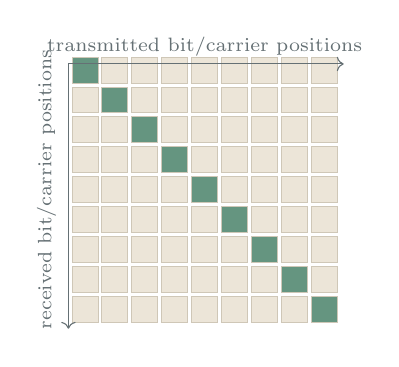
\begin{tikzpicture}[scale=0.38]
        \foreach \i in {0,...,8} {
          \foreach \j in {0,...,8} {
            \node[tinycell,fill=nullc] at (\i,-\j) {};
          }
        }
        \foreach \i in {0,...,8} {
          \node[tinycell,fill=juna!70] at (\i,-\i) {};
        }
        \draw[->,draw=muted] (-0.55,0.2) -- (8.65,0.2);
        \draw[->,draw=muted] (-0.55,0.2) -- (-0.55,-8.65);
        \node[font=\scriptsize,text=muted] at (4.0,0.78) {transmitted bit/carrier positions};
        \node[font=\scriptsize,text=muted,rotate=90] at (-1.28,-4.0) {received bit/carrier positions};
      \end{tikzpicture}
      \vspace{0.05cm}
      {\scriptsize Each received carrier mainly depends on the same transmitted carrier.}
    \end{column}
    \begin{column}{0.49\textwidth}
      \centering
      \textbf{Residual Doppler}\par
      \vspace{0.12cm}
      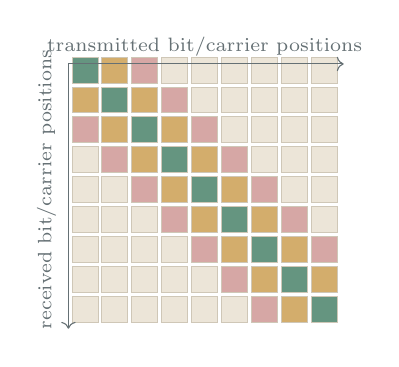
\begin{tikzpicture}[scale=0.38]
        \foreach \i in {0,...,8} {
          \foreach \j in {0,...,8} {
            \node[tinycell,fill=nullc] at (\i,-\j) {};
          }
        }
        \foreach \i in {0,...,8} {
          \node[tinycell,fill=juna!70] at (\i,-\i) {};
        }
        \foreach \i/\j in {1/0,2/1,3/2,4/3,5/4,6/5,7/6,8/7,0/1,1/2,2/3,3/4,4/5,5/6,6/7,7/8} {
          \node[tinycell,fill=gold!70] at (\i,-\j) {};
        }
        \foreach \i/\j in {2/0,3/1,4/2,5/3,6/4,7/5,8/6,0/2,1/3,2/4,3/5,4/6,5/7,6/8} {
          \node[tinycell,fill=rpc!45] at (\i,-\j) {};
        }
        \draw[->,draw=muted] (-0.55,0.2) -- (8.65,0.2);
        \draw[->,draw=muted] (-0.55,0.2) -- (-0.55,-8.65);
        \node[font=\scriptsize,text=muted] at (4.0,0.78) {transmitted bit/carrier positions};
        \node[font=\scriptsize,text=muted,rotate=90] at (-1.28,-4.0) {received bit/carrier positions};
      \end{tikzpicture}
      \vspace{0.05cm}
      {\scriptsize Energy leaks into neighboring carriers; recovery becomes a coupled problem.}
    \end{column}
  \end{columns}
\end{frame}

\begin{frame}{Why clean OFDM has no carrier-to-carrier leakage}
  \vspace{-0.12cm}
  {\small Bin $k$ listens by rotating the received waveform backward at $f_k$ and averaging over one symbol.}
  \vspace{0.14cm}

  \centering
  \resizebox{0.96\linewidth}{!}{%
  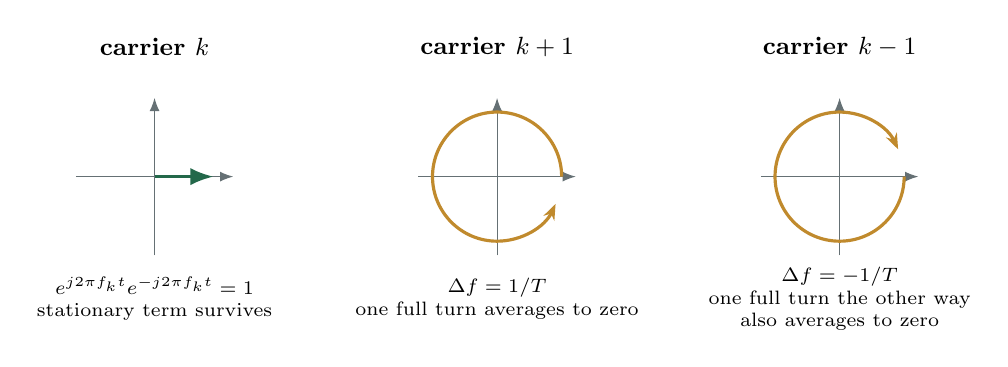
\begin{tikzpicture}[x=1cm,y=1cm,>=Latex]
    % Desired carrier
    \node[font=\small\bfseries] at (0,1.65) {carrier $k$};
    \draw[->,draw=muted] (-1.0,0) -- (1.0,0);
    \draw[->,draw=muted] (0,-1.0) -- (0,1.0);
    \draw[->,draw=juna,line width=1.2pt] (0,0) -- (0.75,0.0);
    \node[font=\scriptsize,align=center] at (0,-1.55)
      {$e^{j2\pi f_k t}e^{-j2\pi f_k t}=1$\\stationary term survives};

    % Neighbor plus
    \begin{scope}[shift={(4.35,0)}]
      \node[font=\small\bfseries] at (0,1.65) {carrier $k+1$};
      \draw[->,draw=muted] (-1.0,0) -- (1.0,0);
      \draw[->,draw=muted] (0,-1.0) -- (0,1.0);
      \draw[draw=gold,line width=1.15pt,-{Stealth[length=2mm]}]
        (0.82,0) arc[start angle=0,end angle=335,radius=0.82];
      \node[font=\scriptsize,align=center] at (0,-1.55)
        {$\Delta f=1/T$\\one full turn averages to zero};
    \end{scope}

    % Neighbor minus
    \begin{scope}[shift={(8.70,0)}]
      \node[font=\small\bfseries] at (0,1.65) {carrier $k-1$};
      \draw[->,draw=muted] (-1.0,0) -- (1.0,0);
      \draw[->,draw=muted] (0,-1.0) -- (0,1.0);
      \draw[draw=gold,line width=1.15pt,-{Stealth[length=2mm]}]
        (0.82,0) arc[start angle=0,end angle=-335,radius=0.82];
      \node[font=\scriptsize,align=center] at (0,-1.55)
        {$\Delta f=-1/T$\\one full turn the other way\\also averages to zero};
    \end{scope}
  \end{tikzpicture}}

  \vspace{0.18cm}
  \begin{callout}
    Orthogonality is just this: after bin-$k$ demodulation, only carrier $k$ is still. Neighbouring carriers make closed loops over the FFT window, so their average is zero.
  \end{callout}
\end{frame}

\begin{frame}{A common phase shift does not create ICI}
  \vspace{-0.12cm}
  {\small A constant phase shift rotates the whole OFDM symbol by the same angle. It does not change the relative spin rates between carriers.}
  \vspace{0.12cm}

  \begin{columns}[T,onlytextwidth]
    \begin{column}{0.50\textwidth}
      \[
        r(t)=e^{j\phi}\sum_\ell d_\ell e^{j2\pi f_\ell t}
      \]
      \vspace{-0.20cm}
      \[
      \begin{aligned}
        y_k
        &= e^{j\phi}\sum_\ell d_\ell
           \int_0^T e^{j2\pi(f_\ell-f_k)t}\,dt\\
        &= e^{j\phi}d_k
      \end{aligned}
      \]
      \vspace{-0.12cm}
      \begin{callout}
        The constellation rotates, but the off-diagonal carrier terms still integrate to zero.
      \end{callout}
    \end{column}

    \begin{column}{0.47\textwidth}
      \centering
      \resizebox{0.92\linewidth}{!}{%
      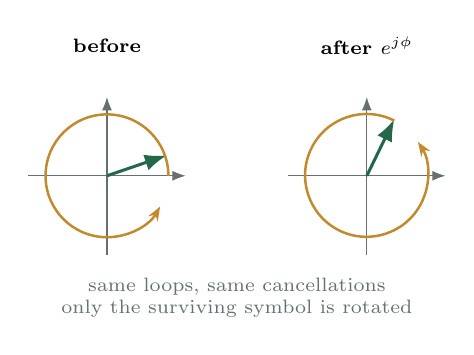
\begin{tikzpicture}[x=1cm,y=1cm,>=Latex]
        \node[font=\scriptsize\bfseries] at (0,1.65) {before};
        \draw[->,draw=muted] (-1.0,0) -- (1.0,0);
        \draw[->,draw=muted] (0,-1.0) -- (0,1.0);
        \draw[->,draw=juna,line width=1.1pt] (0,0) -- (0.76,0.26);
        \draw[draw=gold,line width=0.9pt,-{Stealth[length=1.8mm]}]
          (0.78,0) arc[start angle=0,end angle=330,radius=0.78];

        \begin{scope}[shift={(3.3,0)}]
          \node[font=\scriptsize\bfseries] at (0,1.65) {after $e^{j\phi}$};
          \draw[->,draw=muted] (-1.0,0) -- (1.0,0);
          \draw[->,draw=muted] (0,-1.0) -- (0,1.0);
          \draw[->,draw=juna,line width=1.1pt] (0,0) -- (0.35,0.72);
          \draw[draw=gold,line width=0.9pt,-{Stealth[length=1.8mm]}]
            (0.35,0.70) arc[start angle=63,end angle=393,radius=0.78];
        \end{scope}

        \node[font=\scriptsize,text=muted,align=center] at (1.65,-1.55)
          {same loops, same cancellations\\only the surviving symbol is rotated};
      \end{tikzpicture}}
      \vspace{0.10cm}
      \begin{callout}
        Common phase is a calibration problem, not an orthogonality problem. Pilots can estimate it.
      \end{callout}
    \end{column}
  \end{columns}
\end{frame}

\begin{frame}{Doppler creates ICI by changing the spin rates}
  \vspace{-0.18cm}
  {\footnotesize Each carrier $\ell$, viewed from bin $k$, spins at rate $\Delta f = f_\ell-f_k$. Without Doppler, neighbours spin at exactly $1/T$ and average to zero. Doppler shifts the rate by $\delta_\ell$ \textendash{} the loop no longer closes, and the leftover vector is ICI.}
  \vspace{0.20cm}

  \centering
  \resizebox{0.99\linewidth}{!}{%
  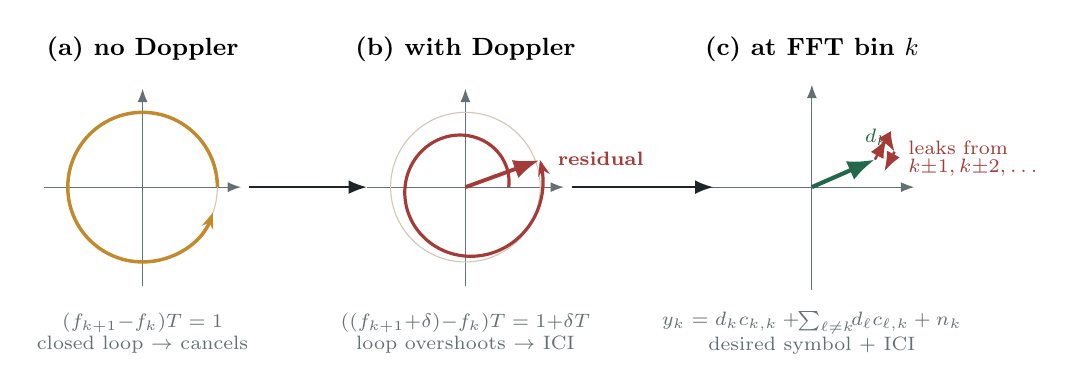
\begin{tikzpicture}[x=1cm,y=1cm,>=Latex]
    % ===== Panel 1: clean neighbour, closes =====
    \node[font=\small\bfseries] at (0,1.75) {(a) no Doppler};
    \draw[->,draw=muted] (-1.25,0) -- (1.25,0);
    \draw[->,draw=muted] (0,-1.25) -- (0,1.25);
    \draw[draw=grid,line width=0.4pt] (0,0) circle (0.95);
    \draw[draw=gold,line width=1.25pt,-{Stealth[length=2mm]}]
      (0.95,0) arc[start angle=0,end angle=340,radius=0.95];
    \node[font=\scriptsize,text=muted,align=center] at (0,-1.85)
      {$(f_{k+1}{-}f_k)T=1$\\closed loop $\rightarrow$ cancels};

    % ===== Panel 2: Doppler-warped, spirals =====
    \begin{scope}[shift={(4.10,0)}]
      \node[font=\small\bfseries] at (0,1.75) {(b) with Doppler};
      \draw[->,draw=muted] (-1.25,0) -- (1.25,0);
      \draw[->,draw=muted] (0,-1.25) -- (0,1.25);
      \draw[draw=grid,line width=0.4pt] (0,0) circle (0.95);
      % outward spiral: radius grows from 0.55 to 1.00 over angle 0..380deg
      \draw[draw=rpc,line width=1.15pt,-{Stealth[length=2mm]}]
        plot[domain=0:380,samples=80,smooth]
          ({(0.55+0.0012*\x)*cos(\x)},{(0.55+0.0012*\x)*sin(\x)});
      % residual = endpoint vector
      \draw[->,draw=rpc,line width=1.4pt] (0,0) -- ({1.00*cos(380)},{1.00*sin(380)});
      \node[font=\scriptsize\bfseries,text=rpc,anchor=south west] at (1.05,0.15) {residual};
      \node[font=\scriptsize,text=muted,align=center] at (0,-1.85)
        {$((f_{k+1}{+}\delta){-}f_k)T=1{+}\delta T$\\loop overshoots $\rightarrow$ ICI};
    \end{scope}

    % ===== Panel 3: bin-k sees a coupled sum =====
    \begin{scope}[shift={(8.50,0)}]
      \node[font=\small\bfseries] at (0,1.75) {(c) at FFT bin $k$};
      \draw[->,draw=muted] (-1.30,0) -- (1.30,0);
      \draw[->,draw=muted] (0,-1.30) -- (0,1.30);
      % desired symbol (big juna arrow)
      \draw[->,draw=juna,line width=1.5pt] (0,0) -- (0.80,0.35);
      \node[font=\scriptsize,text=juna,anchor=south west] at (0.55,0.40) {$d_k$};
      % small leakage residuals being added at tip
      \draw[->,draw=rpc,line width=0.9pt] (0.80,0.35) -- (0.95,0.62);
      \draw[->,draw=rpc,line width=0.9pt] (0.95,0.62) -- (1.05,0.45);
      \draw[->,draw=rpc,line width=0.9pt] (1.05,0.45) -- (0.92,0.20);
      \node[font=\scriptsize,text=rpc,anchor=west] at (1.10,0.50) {leaks from};
      \node[font=\scriptsize,text=rpc,anchor=west] at (1.10,0.25) {$k{\pm}1,k{\pm}2,\ldots$};
      \node[font=\scriptsize,text=muted,align=center] at (0,-1.85)
        {$y_k=d_k c_{k,k}+\!\!\sum_{\ell\ne k}\!\!d_\ell c_{\ell,k}+n_k$\\desired symbol $+$ ICI};
    \end{scope}

    % ===== link arrows =====
    \draw[->,draw=text,line width=0.8pt] (1.35,0) -- (2.85,0);
    \draw[->,draw=text,line width=0.8pt] (5.45,0) -- (7.25,0);
  \end{tikzpicture}}

  \vspace{0.30cm}
  \begin{callout}
    \textbf{One sentence:} Doppler perturbs each carrier's spin rate by $\delta_\ell$, so the FFT's $T$-second average leaves a non-zero residue from every neighbour \textendash{} the receiver hears a \emph{weighted sum} of carriers instead of a single one.
  \end{callout}
\end{frame}

% =====================================================================
% NEW: frequency-domain (sinc) view of ICI
% =====================================================================
\begin{frame}{Same story in the frequency domain: sinc tails leak}
  \vspace{-0.18cm}
  {\footnotesize Each transmitted carrier is a rectangular pulse in time, so it is a $\mathrm{sinc}$ in frequency. The FFT samples the spectrum at the bin centres. Clean OFDM places those samples on every other carrier's \emph{zeros}; Doppler slides the carriers off the grid, so the samples land on the tails.}
  \vspace{0.20cm}

  \begin{columns}[T,onlytextwidth]
    \begin{column}{0.49\textwidth}
      \centering
      \textbf{\small Clean OFDM \textendash{} samples on zeros}\par
      \vspace{0.10cm}
      \resizebox{0.99\linewidth}{!}{%
      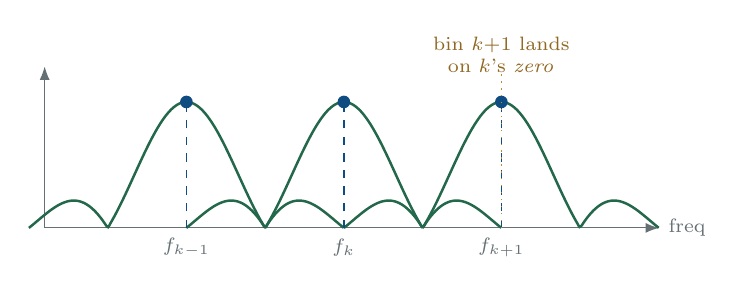
\begin{tikzpicture}[x=1cm,y=1cm,>=Latex]
        % axis
        \draw[->,draw=muted] (-0.3,0) -- (7.5,0) node[right,font=\scriptsize,text=muted] {freq};
        \draw[->,draw=muted] (-0.3,0) -- (-0.3,2.05);
        % three sincs centred at x=1.5, 3.5, 5.5 (spacing = 2 = "1/T")
        \foreach \cx/\col/\lab in {1.5/juna/{$k{-}1$},3.5/juna/{$k$},5.5/juna/{$k{+}1$}} {
          \draw[draw=\col,line width=0.9pt,smooth,samples=160,domain=-2.0:2.0]
            plot ({\cx+\x},{1.6*abs(sin(pi*\x r)/(pi*\x+0.00001))});
        }
        % FFT sample points (drop a vertical at each bin centre)
        \foreach \cx in {1.5,3.5,5.5} {
          \fill[accent] (\cx,1.60) circle (0.08);
          \draw[draw=accent,line width=0.5pt,dashed] (\cx,0) -- (\cx,1.60);
        }
        % labels
        \node[font=\scriptsize,text=muted] at (1.5,-0.25) {$f_{k-1}$};
        \node[font=\scriptsize,text=muted] at (3.5,-0.25) {$f_k$};
        \node[font=\scriptsize,text=muted] at (5.5,-0.25) {$f_{k+1}$};
        % zero-crossing emphasis
        \draw[draw=gold,line width=0.5pt,dotted] (5.5,0) -- (5.5,1.95);
        \node[font=\scriptsize,text=gold!75!black,align=center] at (5.5,2.20)
          {bin $k{+}1$ lands\\on $k$'s \emph{zero}};
      \end{tikzpicture}}
      \vspace{0.10cm}
      \begin{callout}
        \scriptsize Each FFT bin reads only its own carrier. Off-grid tails vanish at every other bin centre.
      \end{callout}
    \end{column}

    \begin{column}{0.49\textwidth}
      \centering
      \textbf{\small With Doppler \textendash{} samples on tails}\par
      \vspace{0.10cm}
      \resizebox{0.99\linewidth}{!}{%
      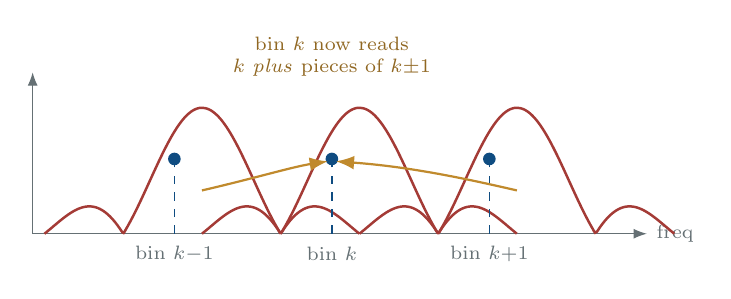
\begin{tikzpicture}[x=1cm,y=1cm,>=Latex]
        \draw[->,draw=muted] (-0.3,0) -- (7.5,0) node[right,font=\scriptsize,text=muted] {freq};
        \draw[->,draw=muted] (-0.3,0) -- (-0.3,2.05);
        % shifted sincs (carriers move right by 0.35)
        \foreach \cx/\col in {1.85/rpc,3.85/rpc,5.85/rpc} {
          \draw[draw=\col,line width=0.9pt,smooth,samples=160,domain=-2.0:2.0]
            plot ({\cx+\x},{1.6*abs(sin(pi*\x r)/(pi*\x+0.00001))});
        }
        % FFT bin centres stay where they were
        \foreach \cx/\h in {1.5/0.95,3.5/0.95,5.5/0.95} {
          \fill[accent] (\cx,\h) circle (0.08);
          \draw[draw=accent,line width=0.5pt,dashed] (\cx,0) -- (\cx,\h);
        }
        \node[font=\scriptsize,text=muted] at (1.5,-0.25) {bin $k{-}1$};
        \node[font=\scriptsize,text=muted] at (3.5,-0.25) {bin $k$};
        \node[font=\scriptsize,text=muted] at (5.5,-0.25) {bin $k{+}1$};
        % highlight bin-k receiving tails from neighbours
        \draw[->,draw=gold,line width=0.8pt] (1.85,0.55) .. controls (2.5,0.7) and (3.0,0.85) .. (3.45,0.92);
        \draw[->,draw=gold,line width=0.8pt] (5.85,0.55) .. controls (5.2,0.7) and (4.5,0.85) .. (3.55,0.92);
        \node[font=\scriptsize,text=gold!75!black,align=center] at (3.5,2.25)
          {bin $k$ now reads\\$k$ \emph{plus} pieces of $k{\pm}1$};
      \end{tikzpicture}}
      \vspace{0.10cm}
      \begin{callout}
        \scriptsize Shifted carriers no longer null at the bin grid. The sinc tails are exactly the ICI coefficients $c_{\ell,k}$.
      \end{callout}
    \end{column}
  \end{columns}
\end{frame}

% =====================================================================
% NEW: synthesis slide -- residuals -> ICI matrix
% =====================================================================
\begin{frame}{From per-carrier residuals to a coupled system}
  \vspace{-0.15cm}
  {\footnotesize Every transmitted carrier leaves a residue in \emph{every} FFT bin. Collect those residues into a matrix and OFDM detection becomes a small linear-algebra problem instead of $N$ independent ones.}
  \vspace{0.20cm}

  \begin{columns}[T,onlytextwidth]
    \begin{column}{0.55\textwidth}
      \centering
      \resizebox{0.99\linewidth}{!}{%
      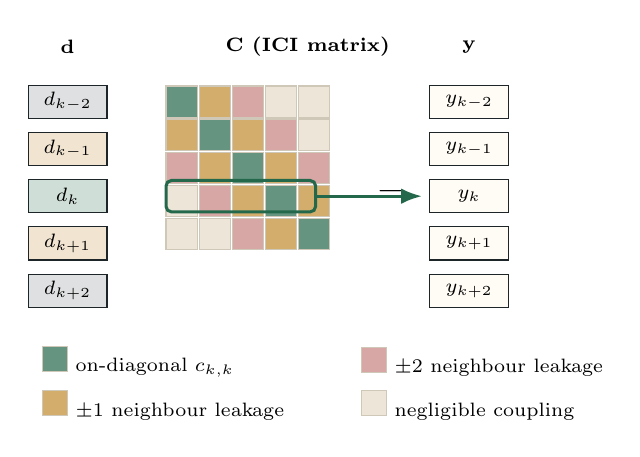
\begin{tikzpicture}[x=1cm,y=1cm,>=Latex]
        % transmitted-symbol column
        \node[font=\scriptsize\bfseries] at (-0.05,3.0) {$\mathbf{d}$};
        \foreach \y/\lab/\col in {2.3/{$d_{k-2}$}/data,1.7/{$d_{k-1}$}/gold,1.1/{$d_k$}/juna,0.5/{$d_{k+1}$}/gold,-0.1/{$d_{k+2}$}/data} {
          \node[draw=text,fill=\col!22,minimum width=1.0cm,minimum height=0.42cm,inner sep=0pt,font=\scriptsize] at (-0.05,\y) {\lab};
        }

        % matrix C
        \node[font=\scriptsize\bfseries] at (3.0,3.0) {$\mathbf{C}$ (ICI matrix)};
        % 5x5 grid: diagonal juna, off-diagonal-1 gold, off-diagonal-2 rpc light
        \foreach \i in {0,...,4} {
          \foreach \j in {0,...,4} {
            \pgfmathsetmacro{\xx}{1.4+\j*0.42}
            \pgfmathsetmacro{\yy}{2.3-\i*0.42}
            \pgfmathtruncatemacro{\d}{abs(\i-\j)}
            \ifnum\d=0
              \node[draw=grid,fill=juna!70,minimum size=0.40cm,inner sep=0pt] at (\xx,\yy) {};
            \else
              \ifnum\d=1
                \node[draw=grid,fill=gold!70,minimum size=0.40cm,inner sep=0pt] at (\xx,\yy) {};
              \else
                \ifnum\d=2
                  \node[draw=grid,fill=rpc!45,minimum size=0.40cm,inner sep=0pt] at (\xx,\yy) {};
                \else
                  \node[draw=grid,fill=nullc,minimum size=0.40cm,inner sep=0pt] at (\xx,\yy) {};
                \fi
              \fi
            \fi
          }
        }

        % equals
        \node[font=\large] at (4.05,1.1) {$=$};

        % received-symbol column y
        \node[font=\scriptsize\bfseries] at (5.05,3.0) {$\mathbf{y}$};
        \foreach \y/\lab in {2.3/{$y_{k-2}$},1.7/{$y_{k-1}$},1.1/{$y_k$},0.5/{$y_{k+1}$},-0.1/{$y_{k+2}$}} {
          \node[draw=text,fill=panel,minimum width=1.0cm,minimum height=0.42cm,inner sep=0pt,font=\scriptsize] at (5.05,\y) {\lab};
        }

        % highlight row k
        \draw[draw=juna,line width=1.1pt,rounded corners=2pt] (1.20,0.90) rectangle (3.10,1.30);
        \draw[->,draw=juna,line width=1pt] (3.10,1.10) -- (4.45,1.10);

        % legend
        \node[font=\scriptsize,anchor=west] at (-0.5,-1.0)
          {\tikz\node[draw=grid,fill=juna!70,minimum size=0.32cm,inner sep=0pt]{}; on-diagonal $c_{k,k}$};
        \node[font=\scriptsize,anchor=west] at (-0.5,-1.55)
          {\tikz\node[draw=grid,fill=gold!70,minimum size=0.32cm,inner sep=0pt]{}; $\pm1$ neighbour leakage};
        \node[font=\scriptsize,anchor=west] at (3.55,-1.0)
          {\tikz\node[draw=grid,fill=rpc!45,minimum size=0.32cm,inner sep=0pt]{}; $\pm2$ neighbour leakage};
        \node[font=\scriptsize,anchor=west] at (3.55,-1.55)
          {\tikz\node[draw=grid,fill=nullc,minimum size=0.32cm,inner sep=0pt]{}; negligible coupling};
      \end{tikzpicture}}
    \end{column}

    \begin{column}{0.43\textwidth}
      \begin{callout}
        \scriptsize\textbf{Where each $c_{\ell,k}$ comes from:} the residual vector from panel (b) of the previous slide \textendash{} or equivalently the sinc-tail value of the previous slide.
      \end{callout}
      \vspace{0.12cm}
      \begin{callout}
        \scriptsize\textbf{Static channel:} $\mathbf{C}$ is diagonal. Each $y_k$ depends only on $d_k$.
      \end{callout}
      \vspace{0.08cm}
      \begin{callout}
        \scriptsize\textbf{Doppler channel:} $\mathbf{C}$ becomes banded. Each $y_k$ sees its desired symbol \emph{plus} a handful of neighbours.
      \end{callout}
      \vspace{0.08cm}
      {\scriptsize\color{muted}\textbf{Receiver's job:} undo the off-diagonal band. RPC does this with pilot-trained partial-FFT weights; JUNA adds LDPC checks as a second anchor.}
    \end{column}
  \end{columns}
\end{frame}

% =====================================================================
% 6. PILOTS AND CHANNELS (was slide 2)
% =====================================================================
\begin{frame}{How the receiver normally orients itself}
  \centering
  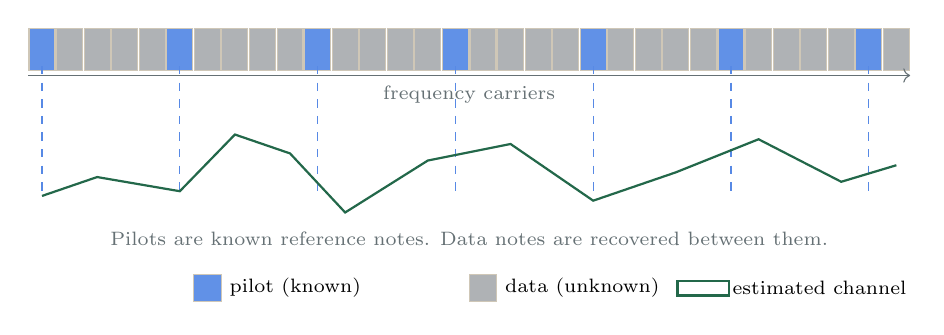
\begin{tikzpicture}[x=0.35cm,y=0.60cm]
    \foreach \i in {0,...,31} {
      \node[draw=grid,fill=data!55,minimum width=0.33cm,minimum height=0.54cm,inner sep=0pt] at (\i,0) {};
    }
    \foreach \i in {0,5,10,15,20,25,30} {
      \node[draw=grid,fill=pilot!75,minimum width=0.33cm,minimum height=0.54cm,inner sep=0pt] at (\i,0) {};
    }
    \draw[->,draw=muted] (-0.5,-0.55) -- (31.5,-0.55);
    \node[font=\scriptsize,text=muted] at (15.5,-0.95) {frequency carriers};
    \foreach \x in {0,5,10,15,20,25,30} {
      \draw[dashed,draw=pilot!80] (\x,-0.35) -- (\x,-3.1);
    }
    \draw[thick,juna] (0,-3.1) -- (2,-2.7) -- (5,-3.0) -- (7,-1.8) -- (9,-2.2)
      -- (11,-3.45) -- (14,-2.35) -- (17,-2.0) -- (20,-3.2) -- (23,-2.6)
      -- (26,-1.9) -- (29,-2.8) -- (31,-2.45);
    \node[font=\scriptsize,text=muted] at (15.5,-4.0)
      {Pilots are known reference notes. Data notes are recovered between them.};
    \node[fill=pilot!75,draw=grid,minimum width=0.35cm,minimum height=0.35cm] at (6.0,-5.05) {};
    \node[font=\scriptsize,anchor=west] at (6.45,-5.05) {pilot (known)};
    \node[fill=data!55,draw=grid,minimum width=0.35cm,minimum height=0.35cm] at (16.0,-5.05) {};
    \node[font=\scriptsize,anchor=west] at (16.45,-5.05) {data (unknown)};
    \node[draw=juna,line width=1pt,minimum width=0.65cm,minimum height=0.18cm,inner sep=0pt] at (24.0,-5.05) {};
    \node[font=\scriptsize,anchor=west] at (24.7,-5.05) {estimated channel};
  \end{tikzpicture}
  \vspace{0.25cm}
  \begin{columns}[T,onlytextwidth]
    \begin{column}{0.31\textwidth}
      \small\textbf{The channel} bends and notches the signal because of echoes off the surface and sea bed.
    \end{column}
    \begin{column}{0.31\textwidth}
      \small\textbf{Pilots} are known anchors. More anchors = better tracking, but less room for payload.
    \end{column}
    \begin{column}{0.31\textwidth}
      \small\textbf{JUNA} adds a third anchor \textendash{} the error-correcting code itself \textendash{} so fewer pilots can do the same job.
    \end{column}
  \end{columns}
\end{frame}

% =====================================================================
% 7. PARTIAL-FFT COMBINING AND JUNA
% =====================================================================
\begin{frame}{Why one long FFT fails under Doppler}
  \vspace{-0.10cm}
  {\small The full FFT assumes the channel is nearly fixed over the whole OFDM symbol. Doppler makes that assumption false.}
  \vspace{0.20cm}

  \begin{columns}[T,onlytextwidth]
    \begin{column}{0.48\textwidth}
      \centering
      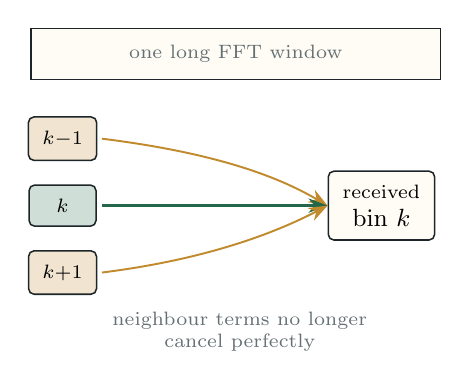
\begin{tikzpicture}[x=1cm,y=1cm,>=Latex]
        \draw[draw=text,fill=panel,line width=0.55pt] (0,1.05) rectangle (5.2,1.70);
        \node[font=\scriptsize,text=muted] at (2.6,1.38) {one long FFT window};
        \foreach \y/\lab/\col in {0.30/{$k{-}1$}/gold,-0.55/{$k$}/juna,-1.40/{$k{+}1$}/gold} {
          \node[block,minimum width=0.85cm,minimum height=0.42cm,fill=\col!22] at (0.40,\y) {\scriptsize \lab};
        }
        \node[block,minimum width=1.35cm,minimum height=0.60cm,fill=panel] (out) at (4.45,-0.55) {\scriptsize received\\[-1pt] bin $k$};
        \draw[arrow,draw=gold] (0.90,0.30) .. controls (2.1,0.15) and (3.0,-0.10) .. (out.west);
        \draw[arrow,draw=juna,line width=1pt] (0.90,-0.55) -- (out.west);
        \draw[arrow,draw=gold] (0.90,-1.40) .. controls (2.1,-1.25) and (3.0,-0.95) .. (out.west);
        \node[font=\scriptsize,text=muted,align=center] at (2.65,-2.15)
          {neighbour terms no longer\\cancel perfectly};
      \end{tikzpicture}
    \end{column}

    \begin{column}{0.49\textwidth}
      \vspace{-0.1cm}
      \[
        y_k =
        \sum_{\ell} d_\ell
        \int_0^T H_\ell(t)\,
        e^{j2\pi(f_\ell-f_k)t}\,dt + n_k
      \]
      \vspace{-0.15cm}
      \begin{callout}
        If $H_\ell(t)$ is constant, the $\ell\ne k$ integrals cancel by orthogonality.
      \end{callout}
      \vspace{0.10cm}
      \begin{callout}
        Under Doppler, $H_\ell(t)$ changes inside the same integral, so leakage remains as ICI.
      \end{callout}
      \vspace{0.12cm}
      {\scriptsize\color{muted}This is the problem partial-FFT demodulation attacks at the receiver front end.}
    \end{column}
  \end{columns}
\end{frame}

% MOVED TO BACKUP: "What viewed from bin k means" and "Carrier ell as seen by bin k" and "Why Df*t is fraction of a turn"
\iffalse
\begin{frame}{What ``viewed from bin $k$'' means}
  \vspace{-0.12cm}
  {\small The FFT bin-$k$ detector listens by multiplying the received signal by bin $k$'s reference wave, $e^{-j2\pi f_k t}$.}
  \vspace{0.16cm}

  \begin{columns}[T,onlytextwidth]
    \begin{column}{0.48\textwidth}
      \centering
      \resizebox{0.96\linewidth}{!}{%
      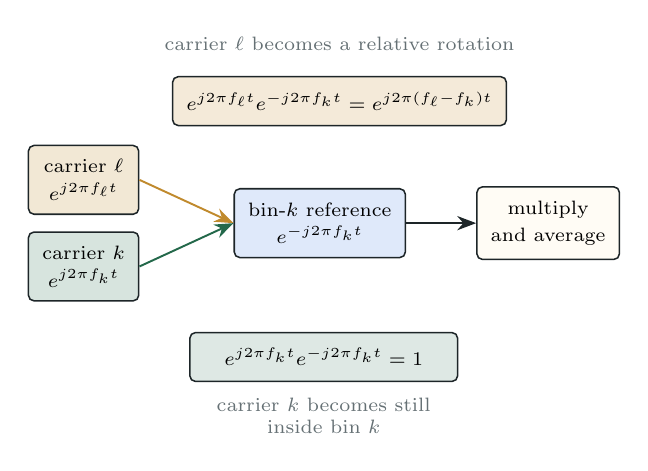
\begin{tikzpicture}[x=1cm,y=1cm,>=Latex]
        \node[block,minimum width=1.40cm,minimum height=0.55cm,fill=gold!20] (ell) at (0,1.05)
          {\scriptsize carrier $\ell$\\[-1pt]\scriptsize $e^{j2\pi f_\ell t}$};
        \node[block,minimum width=1.40cm,minimum height=0.55cm,fill=juna!18] (k) at (0,-0.05)
          {\scriptsize carrier $k$\\[-1pt]\scriptsize $e^{j2\pi f_k t}$};
        \node[block,minimum width=1.70cm,minimum height=0.62cm,fill=pilot!15] (ref) at (3.0,0.50)
          {\scriptsize bin-$k$ reference\\[-1pt]\scriptsize $e^{-j2\pi f_k t}$};
        \node[block,minimum width=1.75cm,minimum height=0.62cm,fill=panel] (mix) at (5.90,0.50)
          {\scriptsize multiply\\[-1pt]\scriptsize and average};

        \draw[arrow,draw=gold] (ell.east) -- (ref.west);
        \draw[arrow,draw=juna] (k.east) -- (ref.west);
        \draw[arrow] (ref.east) -- (mix.west);

        \node[block,minimum width=3.40cm,minimum height=0.62cm,fill=juna!15] (same) at (3.05,-1.20)
          {\scriptsize $e^{j2\pi f_k t}e^{-j2\pi f_k t}=1$};
        \node[font=\scriptsize,text=muted,align=center] at (3.05,-1.95)
          {carrier $k$ becomes still\\inside bin $k$};

        \node[block,minimum width=4.10cm,minimum height=0.62cm,fill=gold!18] (other) at (3.25,2.05)
          {\scriptsize $e^{j2\pi f_\ell t}e^{-j2\pi f_k t}
          = e^{j2\pi(f_\ell-f_k)t}$};
        \node[font=\scriptsize,text=muted,align=center] at (3.25,2.78)
          {carrier $\ell$ becomes a relative rotation};
      \end{tikzpicture}}
    \end{column}

    \begin{column}{0.49\textwidth}
      \vspace{-0.05cm}
      \begin{callout}
        ``Viewed from bin $k$'' means we rotate the whole received signal backward at frequency $f_k$.
      \end{callout}
      \vspace{0.10cm}
      \begin{callout}
        In that rotating coordinate system, carrier $k$ stops moving, because its forward rotation and the bin-$k$ reference cancel exactly.
      \end{callout}
      \vspace{0.10cm}
      \begin{callout}
        Every other carrier is left with only its \emph{difference} from bin $k$: $f_\ell-f_k$.
      \end{callout}
      \vspace{0.14cm}
      {\scriptsize\color{muted}
      The FFT then averages over the symbol. A stationary term survives; a clean rotating neighbour averages away.}
    \end{column}
  \end{columns}
\end{frame}

\begin{frame}{Carrier $\ell$ as seen by bin $k$}
  \vspace{-0.12cm}
  {\small After demodulating with bin $k$, carrier $\ell$ becomes the rotating phasor
  $e^{j2\pi(f_\ell-f_k)t}$. The spin rate is the frequency difference
  $\Delta f=f_\ell-f_k$.}
  \vspace{0.18cm}

  \centering
  \resizebox{0.96\linewidth}{!}{%
  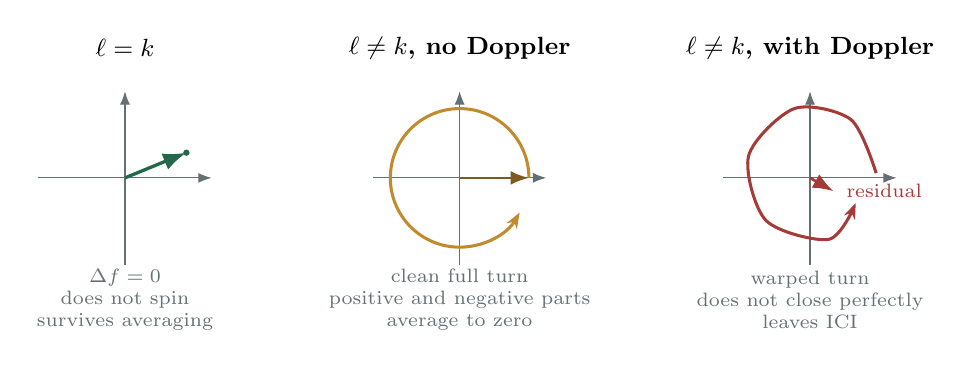
\begin{tikzpicture}[x=1cm,y=1cm,>=Latex]
    % Panel 1: same carrier
    \node[font=\small\bfseries] at (0,1.65) {$\ell=k$};
    \draw[->,draw=muted] (-1.10,0) -- (1.10,0);
    \draw[->,draw=muted] (0,-1.10) -- (0,1.10);
    \draw[->,draw=juna,line width=1.2pt] (0,0) -- (0.78,0.32);
    \fill[juna] (0.78,0.32) circle (0.04);
    \node[font=\scriptsize,text=muted,align=center] at (0,-1.55)
      {$\Delta f=0$\\does not spin\\survives averaging};

    % Panel 2: clean neighbor
    \begin{scope}[shift={(4.25,0)}]
      \node[font=\small\bfseries] at (0,1.65) {$\ell\ne k$, no Doppler};
      \draw[->,draw=muted] (-1.10,0) -- (1.10,0);
      \draw[->,draw=muted] (0,-1.10) -- (0,1.10);
      \draw[draw=gold,line width=1.1pt,-{Stealth[length=2mm]}]
        (0.88,0) arc[start angle=0,end angle=330,radius=0.88];
      \draw[->,draw=gold!65!black,line width=0.8pt] (0,0) -- (0.88,0);
      \node[font=\scriptsize,text=muted,align=center] at (0,-1.55)
        {clean full turn\\positive and negative parts\\average to zero};
    \end{scope}

    % Panel 3: Doppler-warped neighbor
    \begin{scope}[shift={(8.70,0)}]
      \node[font=\small\bfseries] at (0,1.65) {$\ell\ne k$, with Doppler};
      \draw[->,draw=muted] (-1.10,0) -- (1.10,0);
      \draw[->,draw=muted] (0,-1.10) -- (0,1.10);
      \draw[draw=rpc,line width=1.1pt,-{Stealth[length=2mm]}]
        plot[smooth] coordinates {(0.84,0.06) (0.52,0.74) (-0.20,0.88) (-0.78,0.28) (-0.56,-0.54) (0.24,-0.78) (0.58,-0.32)};
      \draw[->,draw=rpc,line width=1pt] (0,0) -- (0.30,-0.17);
      \node[font=\scriptsize,text=rpc,anchor=west] at (0.34,-0.17) {residual};
      \node[font=\scriptsize,text=muted,align=center] at (0,-1.55)
        {warped turn\\does not close perfectly\\leaves ICI};
    \end{scope}
  \end{tikzpicture}}

  \vspace{0.18cm}
  \begin{callout}
    Partial FFT samples this rotation in short windows; RPC chooses weights that rotate the carrier-$k$ pieces back into alignment and reduce the leftover neighbour vectors.
  \end{callout}
\end{frame}

\begin{frame}{Why $\Delta f\,t$ is the fraction of a turn}
  \vspace{-0.12cm}
  {\small Frequency is a rotation rate. Once carrier $\ell$ is viewed from bin $k$,
  the relative rate is $\Delta f=f_\ell-f_k$ cycles per second.}
  \vspace{0.16cm}

  \begin{columns}[T,onlytextwidth]
    \begin{column}{0.47\textwidth}
      \centering
      \resizebox{\linewidth}{!}{%
      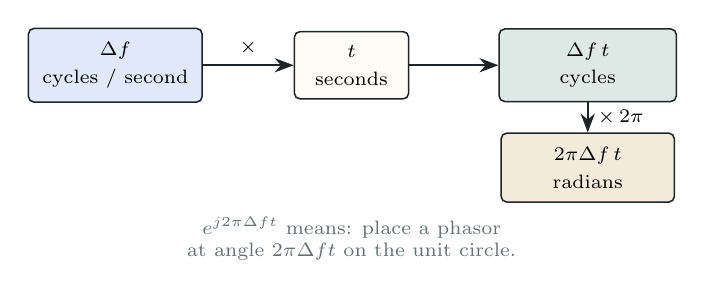
\begin{tikzpicture}[x=1cm,y=1cm,>=Latex]
        \node[block,minimum width=2.1cm,minimum height=0.62cm,fill=pilot!15] (rate) at (0,1.2)
          {\scriptsize $\Delta f$\\[-1pt]\scriptsize cycles / second};
        \node[block,minimum width=1.45cm,minimum height=0.62cm,fill=panel] (time) at (3.0,1.2)
          {\scriptsize $t$\\[-1pt]\scriptsize seconds};
        \node[block,minimum width=2.25cm,minimum height=0.62cm,fill=juna!15] (cycles) at (6.0,1.2)
          {\scriptsize $\Delta f\,t$\\[-1pt]\scriptsize cycles};
        \node[block,minimum width=2.2cm,minimum height=0.62cm,fill=gold!18] (phase) at (6.0,-0.1)
          {\scriptsize $2\pi\Delta f\,t$\\[-1pt]\scriptsize radians};
        \draw[arrow] (rate.east) -- node[font=\scriptsize,above] {$\times$} (time.west);
        \draw[arrow] (time.east) -- (cycles.west);
        \draw[arrow] (cycles.south) -- node[font=\scriptsize,right] {$\times\,2\pi$} (phase.north);
        \node[font=\scriptsize,text=muted,align=center] at (3.0,-1.0)
          {$e^{j2\pi\Delta f t}$ means: place a phasor\\at angle $2\pi\Delta f t$ on the unit circle.};
      \end{tikzpicture}}
    \end{column}

    \begin{column}{0.50\textwidth}
      \centering
      \resizebox{0.92\linewidth}{!}{%
      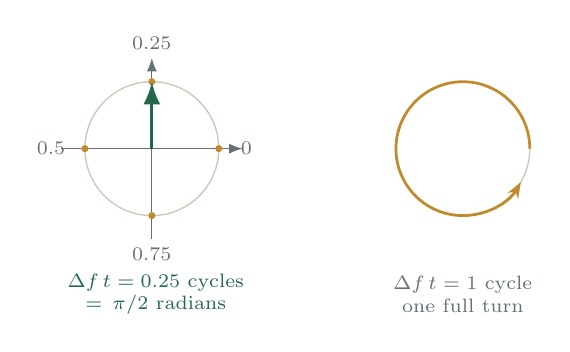
\begin{tikzpicture}[x=1cm,y=1cm,>=Latex]
        \draw[->,draw=muted] (-1.15,0) -- (1.15,0);
        \draw[->,draw=muted] (0,-1.15) -- (0,1.15);
        \draw[draw=grid,line width=0.5pt] (0,0) circle (0.85);
        \fill[gold] (0.85,0) circle (0.045);
        \fill[gold] (0,0.85) circle (0.045);
        \fill[gold] (-0.85,0) circle (0.045);
        \fill[gold] (0,-0.85) circle (0.045);
        \node[font=\scriptsize,text=muted] at (1.20,0) {0};
        \node[font=\scriptsize,text=muted] at (0,1.34) {0.25};
        \node[font=\scriptsize,text=muted] at (-1.28,0) {0.5};
        \node[font=\scriptsize,text=muted] at (0,-1.34) {0.75};
        \draw[->,draw=juna,line width=1.15pt] (0,0) -- (0,0.85);
        \node[font=\scriptsize,text=juna,align=center] at (0.05,-1.85)
          {$\Delta f\,t=0.25$ cycles\\$=\,\pi/2$ radians};

        \begin{scope}[shift={(3.95,0)}]
          \draw[draw=grid,line width=0.5pt] (0,0) circle (0.85);
          \draw[draw=gold,line width=1pt,-{Stealth[length=2mm]}]
            (0.85,0) arc[start angle=0,end angle=330,radius=0.85];
          \node[font=\scriptsize,text=muted,align=center] at (0,-1.85)
            {$\Delta f\,t=1$ cycle\\one full turn};
        \end{scope}
      \end{tikzpicture}}
    \end{column}
  \end{columns}

  \vspace{0.10cm}
  \begin{callout}
    OFDM chooses adjacent carrier spacing $\Delta f=1/T$. Over one FFT window,
    $\Delta f\,T=1$, so a clean neighbour makes exactly one full relative turn and averages to zero.
  \end{callout}
\end{frame}
\fi
% END BACKUP-ONLY BLOCK

\begin{frame}{Chopping preserves information the full FFT throws away}
  \vspace{-0.12cm}
  {\small A full FFT immediately collapses the whole symbol into one number per carrier. Partial FFT delays that collapse.}
  \vspace{0.14cm}

  \begin{columns}[T,onlytextwidth]
    \begin{column}{0.47\textwidth}
      \centering
      \textbf{\small Full FFT: collapse first}\par
      \vspace{0.10cm}
      \resizebox{0.95\linewidth}{!}{%
      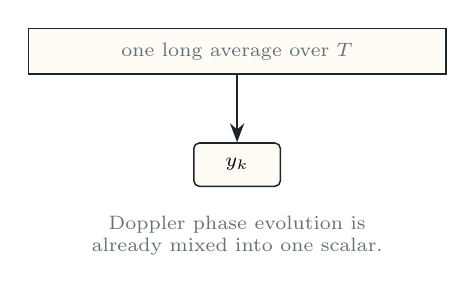
\begin{tikzpicture}[x=1cm,y=1cm,>=Latex]
        \draw[draw=text,fill=panel,line width=0.55pt] (0,1.0) rectangle (5.3,1.58);
        \node[font=\scriptsize,text=muted] at (2.65,1.29) {one long average over $T$};
        \node[block,minimum width=1.10cm,minimum height=0.55cm,fill=panel] (yk) at (2.65,-0.15)
          {\scriptsize $y_k$};
        \draw[arrow] (2.65,1.0) -- (yk.north);
        \node[font=\scriptsize,text=muted,align=center] at (2.65,-1.05)
          {Doppler phase evolution is\\already mixed into one scalar.};
      \end{tikzpicture}}
      \vspace{0.06cm}
      \begin{callout}
        Once this number is formed, the receiver cannot see how the phase changed across the symbol.
      \end{callout}
    \end{column}

    \begin{column}{0.50\textwidth}
      \centering
      \textbf{\small Partial FFT: keep $M$ views first}\par
      \vspace{0.10cm}
      \resizebox{0.95\linewidth}{!}{%
      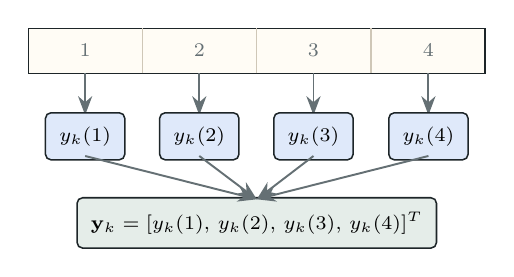
\begin{tikzpicture}[x=1cm,y=1cm,>=Latex]
        \draw[draw=text,fill=panel,line width=0.55pt] (0,1.15) rectangle (5.8,1.72);
        \foreach \x in {1.45,2.90,4.35} {\draw[draw=grid] (\x,1.15) -- (\x,1.72);}
        \foreach \x/\lab in {0.72/1,2.17/2,3.62/3,5.08/4}
          {\node[font=\scriptsize,text=muted] at (\x,1.44) {\lab};}
        \foreach \x/\lab in {0.72/{y_k(1)},2.17/{y_k(2)},3.62/{y_k(3)},5.08/{y_k(4)}} {
          \draw[arrow,draw=muted] (\x,1.15) -- (\x,0.62);
          \node[block,minimum width=0.92cm,minimum height=0.45cm,fill=pilot!15] at (\x,0.35) {\scriptsize $\lab$};
        }
        \node[block,minimum width=4.5cm,minimum height=0.55cm,fill=juna!12] at (2.90,-0.75)
          {\scriptsize $\mathbf{y}_k=[y_k(1),\,y_k(2),\,y_k(3),\,y_k(4)]^T$};
        \foreach \x in {0.72,2.17,3.62,5.08}
          {\draw[arrow,draw=muted] (\x,0.10) -- (2.90,-0.45);}
      \end{tikzpicture}}
      \vspace{0.06cm}
      \begin{callout}
        The vector still contains the branch-to-branch Doppler pattern, so the receiver can choose how to collapse it.
      \end{callout}
    \end{column}
  \end{columns}

  \vspace{0.10cm}
  \centering
  {\scriptsize\color{muted}The gain is not from chopping alone. The gain is from preserving the pattern before combining.}
\end{frame}

\begin{frame}{Weights choose which pattern survives}
  \vspace{-0.15cm}
  {\small Across the partial-FFT branches, the desired carrier and the leaked neighbours have different patterns.}
  \vspace{0.10cm}

  \begin{columns}[T,onlytextwidth]
    \begin{column}{0.48\textwidth}
      \[
        \mathbf{y}_k
        =
        d_k\mathbf{c}_{k,k}
        + d_{k-1}\mathbf{c}_{k-1,k}
        + d_{k+1}\mathbf{c}_{k+1,k}
        + \mathbf{n}_k
      \]
      \vspace{-0.15cm}
      \[
        x_k=\mathbf{w}_k^H\mathbf{y}_k
      \]
      \vspace{-0.15cm}
      \begin{callout}
        The weights are chosen so
        \[
          \mathbf{w}_k^H\mathbf{c}_{k,k}\approx 1
        \]
        desired carrier $k$ adds coherently.
      \end{callout}
      \vspace{0.08cm}
      \begin{callout}
        At the same time,
        \[
          \mathbf{w}_k^H\mathbf{c}_{k\pm1,k}\approx 0
        \]
        neighbour leakage is projected down.
      \end{callout}
    \end{column}

    \begin{column}{0.49\textwidth}
      \centering
      \resizebox{0.95\linewidth}{!}{%
      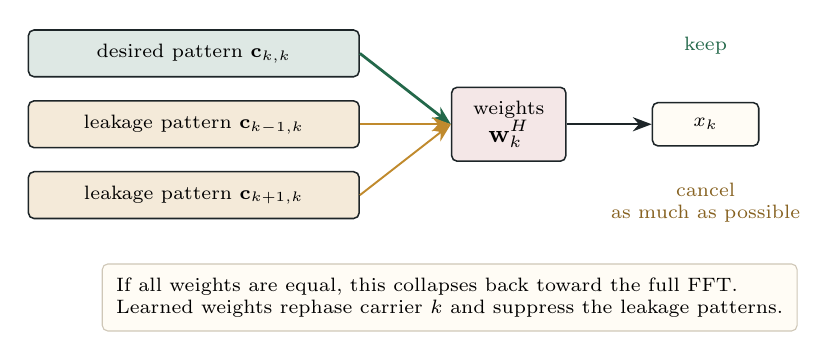
\begin{tikzpicture}[x=1cm,y=1cm,>=Latex]
        \node[block,minimum width=4.2cm,minimum height=0.52cm,fill=juna!15] (good) at (0,1.55)
          {\scriptsize desired pattern $\mathbf{c}_{k,k}$};
        \node[block,minimum width=4.2cm,minimum height=0.52cm,fill=gold!18] (leak1) at (0,0.65)
          {\scriptsize leakage pattern $\mathbf{c}_{k-1,k}$};
        \node[block,minimum width=4.2cm,minimum height=0.52cm,fill=gold!18] (leak2) at (0,-0.25)
          {\scriptsize leakage pattern $\mathbf{c}_{k+1,k}$};
        \node[block,minimum width=1.45cm,minimum height=0.62cm,fill=rpc!12] (w) at (4.0,0.65)
          {\scriptsize weights\\[-1pt] $\mathbf{w}_k^H$};
        \node[block,minimum width=1.35cm,minimum height=0.55cm,fill=panel] (out) at (6.5,0.65)
          {\scriptsize $x_k$};
        \draw[arrow,draw=juna,line width=1pt] (good.east) -- (w.west);
        \draw[arrow,draw=gold] (leak1.east) -- (w.west);
        \draw[arrow,draw=gold] (leak2.east) -- (w.west);
        \draw[arrow] (w.east) -- (out.west);
        \node[font=\scriptsize,text=juna,align=center] at (6.5,1.65)
          {keep};
        \node[font=\scriptsize,text=gold!70!black,align=center] at (6.5,-0.35)
          {cancel\\as much as possible};

        \node[draw=grid,fill=panel,rounded corners=2pt,inner sep=5pt,align=left,font=\scriptsize]
          at (3.25,-1.55) {If all weights are equal, this collapses back toward the full FFT.\\
          Learned weights rephase carrier $k$ and suppress the leakage patterns.};
      \end{tikzpicture}}
      \vspace{0.10cm}
      \begin{callout}
        This is like beamforming, but the ``sensors'' are time slices instead of microphones.
      \end{callout}
    \end{column}
  \end{columns}
\end{frame}

\begin{frame}{Partial FFT keeps the Doppler pattern visible}
  \vspace{-0.12cm}
  {\small Instead of collapsing the whole symbol into one number per carrier, partial FFT keeps $M$ short-window measurements.}
  \vspace{0.14cm}

  \begin{columns}[T,onlytextwidth]
    \begin{column}{0.53\textwidth}
      \centering
      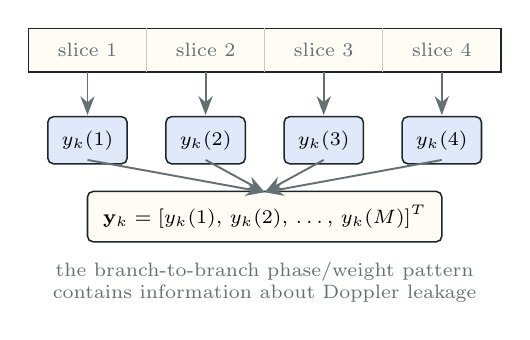
\begin{tikzpicture}[x=1cm,y=1cm,>=Latex]
        \draw[draw=text,fill=panel,line width=0.55pt] (0,2.0) rectangle (6.0,2.55);
        \foreach \x in {1.5,3.0,4.5} {\draw[draw=grid] (\x,2.0) -- (\x,2.55);}
        \foreach \x/\lab in {0.75/1,2.25/2,3.75/3,5.25/4}
          {\node[font=\scriptsize,text=muted] at (\x,2.28) {slice \lab};}

        \foreach \x/\lab in {0.75/{y_k(1)},2.25/{y_k(2)},3.75/{y_k(3)},5.25/{y_k(4)}} {
          \draw[arrow,draw=muted] (\x,2.0) -- (\x,1.45);
          \node[block,minimum width=1.0cm,minimum height=0.46cm,fill=pilot!15] at (\x,1.13) {\scriptsize $\lab$};
        }

        \node[block,minimum width=4.5cm,minimum height=0.62cm,fill=panel] at (3.0,0.16)
          {\scriptsize $\mathbf{y}_k=[y_k(1),\,y_k(2),\,\ldots,\,y_k(M)]^T$};
        \foreach \x in {0.75,2.25,3.75,5.25}
          {\draw[arrow,draw=muted] (\x,0.88) -- (3.0,0.47);}

        \node[font=\scriptsize,text=muted,align=center] at (3.0,-0.67)
          {the branch-to-branch phase/weight pattern\\contains information about Doppler leakage};
      \end{tikzpicture}
    \end{column}

    \begin{column}{0.44\textwidth}
      \[
        y_k(m) \approx
        \sum_{\ell} d_\ell H_\ell(m) I_{\ell-k}(m)
        + n_k(m)
      \]
      \vspace{-0.25cm}
      \[
        \mathbf{y}_k
        =
        \sum_{\ell} d_\ell\,\mathbf{c}_{\ell,k}
        + \mathbf{n}_k
      \]
      \vspace{-0.10cm}
      \begin{callout}
        Each short interval is closer to time-invariant, so the received carrier is less smeared before combining.
      \end{callout}
      \vspace{0.10cm}
      \begin{callout}
        For UWA time-scaling, carrier $k$ has a Doppler phase progression across slices, roughly set by $\epsilon_k=a f_kT$.
      \end{callout}
    \end{column}
  \end{columns}
\end{frame}

\begin{frame}{RPC weights align carrier $k$ and suppress leakage}
  \vspace{-0.12cm}
  {\small The partial-FFT branches are combined with a carrier-specific vector $\mathbf{w}_k$. The weights act like a stepwise receiver window.}
  \vspace{0.12cm}

  \begin{columns}[T,onlytextwidth]
    \begin{column}{0.48\textwidth}
      \centering
      \resizebox{\linewidth}{!}{%
      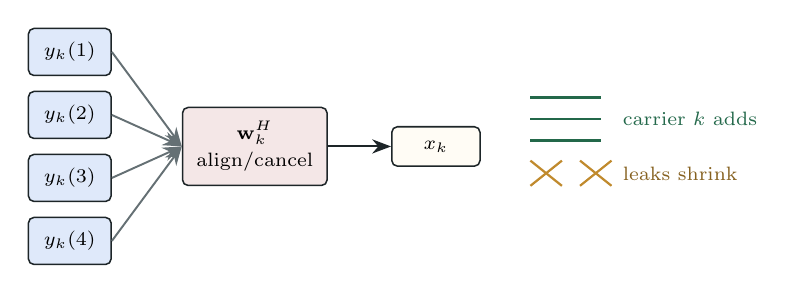
\begin{tikzpicture}[x=1cm,y=1cm,>=Latex]
        \node[block,minimum width=1.05cm,minimum height=0.48cm,fill=pilot!15] (y1) at (0,1.20) {\scriptsize $y_k(1)$};
        \node[block,minimum width=1.05cm,minimum height=0.48cm,fill=pilot!15] (y2) at (0,0.40) {\scriptsize $y_k(2)$};
        \node[block,minimum width=1.05cm,minimum height=0.48cm,fill=pilot!15] (y3) at (0,-0.40) {\scriptsize $y_k(3)$};
        \node[block,minimum width=1.05cm,minimum height=0.48cm,fill=pilot!15] (y4) at (0,-1.20) {\scriptsize $y_k(4)$};

        \node[block,minimum width=1.55cm,minimum height=0.62cm,fill=rpc!12] (w) at (2.35,0.0) {\scriptsize $\mathbf{w}_k^H$\\[-1pt]\scriptsize align/cancel};
        \node[block,minimum width=1.12cm,minimum height=0.50cm,fill=panel] (x) at (4.65,0.0) {\scriptsize $x_k$};
        \foreach \n in {y1,y2,y3,y4} {\draw[arrow,draw=muted] (\n.east) -- (w.west);}
        \draw[arrow] (w.east) -- (x.west);

        \draw[draw=juna,line width=1pt] (5.85,0.62) -- (6.75,0.62);
        \draw[draw=juna,line width=1pt] (5.85,0.35) -- (6.75,0.35);
        \draw[draw=juna,line width=1pt] (5.85,0.08) -- (6.75,0.08);
        \node[font=\scriptsize,anchor=west,text=juna] at (6.90,0.35) {carrier $k$ adds};

        \draw[draw=gold,line width=0.8pt] (5.85,-0.50) -- (6.25,-0.18);
        \draw[draw=gold,line width=0.8pt] (6.25,-0.50) -- (5.85,-0.18);
        \draw[draw=gold,line width=0.8pt] (6.48,-0.50) -- (6.88,-0.18);
        \draw[draw=gold,line width=0.8pt] (6.88,-0.50) -- (6.48,-0.18);
        \node[font=\scriptsize,anchor=west,text=gold!70!black] at (6.90,-0.35) {leaks shrink};
      \end{tikzpicture}}
    \end{column}

    \begin{column}{0.49\textwidth}
      \footnotesize
      \setlength{\abovedisplayskip}{0.35em}
      \setlength{\belowdisplayskip}{0.35em}
      \[
      \begin{aligned}
        x_k&=\mathbf{w}_k^H\mathbf{y}_k\\
            &= d_k a_{k,k}
             + \sum_{\ell\ne k} d_\ell a_{\ell,k}
             + \tilde n_k
      \end{aligned}
      \]
      \[
        a_{\ell,k}=\mathbf{w}_k^H\mathbf{c}_{\ell,k},
        \qquad
        a_{k,k}\approx 1,\quad a_{\ell,k}\approx 0
      \]
      \begin{callout}
        With a time-scaling model, the weights undo the Doppler phase across slices before one-tap equalisation. RPC learns them from pilots and decisions; JUNA adds LDPC constraints.
      \end{callout}
    \end{column}
  \end{columns}
\end{frame}

\begin{frame}{Partial-FFT combining: separating carriers that now talk to each other}
  \vspace{-0.12cm}
  {\scriptsize RPC mitigates Doppler by using short partial FFTs: each slice is closer to time-invariant, and $\mathbf{w}_k$ aligns carrier $k$ while partly nulling neighbour leakage.}
  \vspace{0.08cm}

  \begin{columns}[T,onlytextwidth]
    % ---------- Panel 1: the problem ----------
    \begin{column}{0.30\textwidth}
      \centering
      \textbf{\small 1.\ One FFT $=$ local mixture}\par
      \vspace{0.18cm}
      \resizebox{0.95\linewidth}{!}{%
      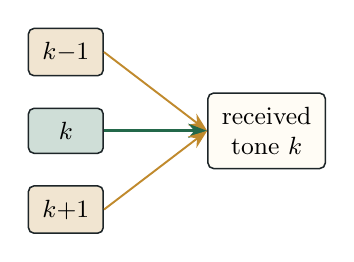
\begin{tikzpicture}[x=1cm,y=1cm,>=Latex]
        \node[block,minimum width=0.95cm,minimum height=0.55cm,fill=gold!22] (km) at (0,1.0) {\small$k{-}1$};
        \node[block,minimum width=0.95cm,minimum height=0.55cm,fill=juna!22] (k)  at (0,0.0) {\small$k$};
        \node[block,minimum width=0.95cm,minimum height=0.55cm,fill=gold!22] (kp) at (0,-1.0) {\small$k{+}1$};
        \node[block,minimum width=1.40cm,minimum height=0.75cm,fill=panel] (yk) at (2.55,0.0) {\small received\\\small tone $k$};
        \draw[arrow,draw=gold] (km.east) -- (yk.west);
        \draw[arrow,draw=juna,line width=1.0pt] (k.east) -- (yk.west);
        \draw[arrow,draw=gold] (kp.east) -- (yk.west);
      \end{tikzpicture}}
      \vspace{0.10cm}
      \parbox{\linewidth}{\centering\scriptsize Tone $k$ is contaminated mainly by its immediate neighbours.}
    \end{column}

    % ---------- Panel 2: partial FFT ----------
    \begin{column}{0.40\textwidth}
      \centering
      \textbf{\small 2.\ Partial FFT $=$ $M$ views per tone}\par
      \vspace{0.12cm}
      \resizebox{0.88\linewidth}{!}{%
      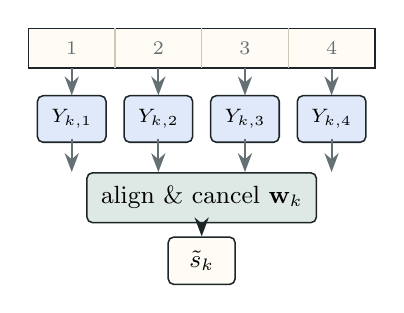
\begin{tikzpicture}[x=1cm,y=1cm,>=Latex]
        % time-sliced symbol bar
        \draw[draw=text,fill=panel,line width=0.55pt] (0,1.30) rectangle (4.4,1.80);
        \foreach \x in {1.10,2.20,3.30} {\draw[draw=grid] (\x,1.30) -- (\x,1.80);}
        \foreach \x/\lab in {0.55/1,1.65/2,2.75/3,3.85/4}
          {\node[font=\scriptsize,text=muted] at (\x,1.55) {\lab};}

        % four aligned partial outputs
        \foreach \x/\lab in {0.55/{Y_{k,1}},1.65/{Y_{k,2}},2.75/{Y_{k,3}},3.85/{Y_{k,4}}} {
          \draw[arrow,draw=muted] (\x,1.30) -- (\x,0.95);
          \node[block,minimum width=0.80cm,minimum height=0.50cm,fill=pilot!15] at (\x,0.65) {\scriptsize $\lab$};
        }

        % combiner
        \node[block,minimum width=1.85cm,minimum height=0.60cm,fill=juna!15] (comb) at (2.20,-0.35)
          {\small align \& cancel $\mathbf{w}_k$};
        \foreach \x in {0.55,1.65,2.75,3.85}
          {\draw[arrow,draw=muted] (\x,0.40) -- (comb.north -| {\x,0});}

        % output
        \node[block,minimum width=0.85cm,minimum height=0.50cm,fill=panel] (s) at (2.20,-1.15) {\small $\tilde{s}_k$};
        \draw[arrow] (comb.south) -- (s.north);
      \end{tikzpicture}}
      \vspace{0.02cm}
      \parbox{\linewidth}{\centering\scriptsize Short windows make Doppler look almost constant; the branch pattern exposes the leakage.}
    \end{column}

    % ---------- Panel 3: who chooses the weights ----------
    \begin{column}{0.28\textwidth}
      \centering
      \textbf{\small 3.\ Who chooses $\mathbf{w}_k$?}\par
      \vspace{0.18cm}
      \resizebox{0.95\linewidth}{!}{%
      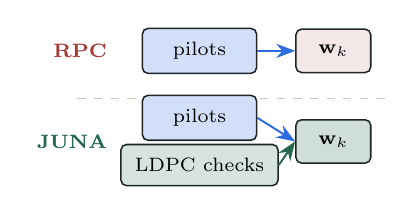
\begin{tikzpicture}[x=1cm,y=1cm,>=Latex]
        % RPC row
        \node[font=\scriptsize\bfseries,text=rpc,anchor=east] at (-0.1,1.15) {RPC};
        \node[block,minimum width=1.45cm,minimum height=0.55cm,fill=pilot!22] (rpil) at (0.95,1.15) {\scriptsize pilots};
        \node[block,minimum width=0.95cm,minimum height=0.55cm,fill=rpc!12] (rw)  at (2.65,1.15) {\scriptsize $\mathbf{w}_k$};
        \draw[arrow,draw=pilot] (rpil.east) -- (rw.west);

        % divider
        \draw[draw=grid,dashed] (-0.6,0.55) -- (3.3,0.55);

        % JUNA row
        \node[font=\scriptsize\bfseries,text=juna,anchor=east] at (-0.1,0.0) {JUNA};
        \node[block,minimum width=1.45cm,minimum height=0.45cm,fill=pilot!22] (jpil)  at (0.95,0.30) {\scriptsize pilots};
        \node[block,minimum width=1.45cm,minimum height=0.45cm,fill=juna!18]  (jcode) at (0.95,-0.30) {\scriptsize LDPC checks};
        \node[block,minimum width=0.95cm,minimum height=0.55cm,fill=juna!22]  (jw)    at (2.65,0.0) {\scriptsize $\mathbf{w}_k$};
        \draw[arrow,draw=pilot] (jpil.east) -- (jw.west);
        \draw[arrow,draw=juna]  (jcode.east) -- (jw.west);
      \end{tikzpicture}}
      \vspace{0.02cm}
      \parbox{\linewidth}{\centering\scriptsize RPC learns $\mathbf{w}_k$ from pilots to align $k$ and suppress leaks. JUNA adds LDPC checks as a second anchor.}
    \end{column}
  \end{columns}
\end{frame}

% =====================================================================
% 8-12. THE FIVE CHANNELS
% =====================================================================
\begin{frame}{Channel A \textendash{} an ``easy'' link (200~m, shallow)}
  \channelimage{figs/profile_095_range200m_bathy30m_tx15m_rx15m_bottom_rigid_surface_windy_bounces_3_fs24000_snr_curve_strict_cpp_yuna_smoothed.png}
  \vspace{0.20cm}
  \begin{columns}[T,onlytextwidth]
    \begin{column}{0.46\textwidth}
      \small\textbf{Setup.} 200~m range, 30~m deep, mild echoes, breezy surface.
    \end{column}
    \begin{column}{0.50\textwidth}
      \small\textbf{Read it.} Without motion, both receivers do fine. With motion, RPC's error rate plateaus much higher; JUNA pushes the floor down. \\\textbf{\color{juna} JUNA delivers $\sim$4$\times$ fewer residual errors.}
    \end{column}
  \end{columns}
\end{frame}

\begin{frame}{Channel B \textendash{} longer range, more selective (400~m)}
  \channelimage{figs/profile_049_range400m_bathy30m_tx15m_rx10m_bottom_pressure_release_surface_rigid_bounces_3_fs24000_snr_curve_strict_cpp_yuna_smoothed.png}
  \vspace{0.20cm}
  \begin{columns}[T,onlytextwidth]
    \begin{column}{0.46\textwidth}
      \small\textbf{Setup.} 400~m range, soft bottom, smoother surface. The channel has deeper notches \textendash{} entire frequencies are nearly silent.
    \end{column}
    \begin{column}{0.50\textwidth}
      \small\textbf{Read it.} Even with strong selectivity, JUNA's use of code structure recovers what pilots alone cannot. \\\textbf{\color{juna} JUNA delivers $\sim$3.8$\times$ fewer residual errors.}
    \end{column}
  \end{columns}
\end{frame}

\begin{frame}{Channel C \textendash{} mid-range with deep notches (500~m)}
  \channelimage{figs/profile_038_range500m_bathy30m_tx15m_rx15m_bottom_pressure_release_surface_windy_bounces_3_fs24000_snr_curve_strict_cpp_yuna_smoothed.png}
  \vspace{0.20cm}
  \begin{columns}[T,onlytextwidth]
    \begin{column}{0.46\textwidth}
      \small\textbf{Setup.} 500~m range, windy surface, soft bottom. Deep frequency notches \textendash{} a harder static channel.
    \end{column}
    \begin{column}{0.50\textwidth}
      \small\textbf{Read it.} The baseline is already working harder. JUNA still extracts a meaningful gain. \\\textbf{\color{juna} JUNA delivers $\sim$3.3$\times$ fewer residual errors.}
    \end{column}
  \end{columns}
\end{frame}

\begin{frame}{Channel D \textendash{} shallow, near-surface ducting (300~m)}
  \channelimage{figs/profile_120_range300m_bathy40m_tx5m_rx5m_bottom_pressure_release_surface_rigid_bounces_3_fs24000_snr_curve_strict_cpp_yuna_smoothed.png}
  \vspace{0.20cm}
  \begin{columns}[T,onlytextwidth]
    \begin{column}{0.46\textwidth}
      \small\textbf{Setup.} 300~m range in 40~m water, both nodes near the surface. Lots of close echoes mixing with motion.
    \end{column}
    \begin{column}{0.50\textwidth}
      \small\textbf{Read it.} The error floor is higher overall \textendash{} this is a genuinely difficult channel. JUNA still helps, but the margin narrows. \\\textbf{\color{juna} JUNA delivers $\sim$1.3$\times$ fewer residual errors.}
    \end{column}
  \end{columns}
\end{frame}

\begin{frame}{Channel E \textendash{} the hard wall (100~m, heavy motion mixing)}
  \channelimage{figs/profile_111_range100m_bathy30m_tx15m_rx10m_bottom_pressure_release_surface_pressure_release_bounces_3_fs24000_snr_curve_strict_cpp_yuna_smoothed.png}
  \vspace{0.20cm}
  \begin{columns}[T,onlytextwidth]
    \begin{column}{0.46\textwidth}
      \small\textbf{Setup.} 100~m range, reflective surface and bottom. Carrier-to-carrier interference dominates.
    \end{column}
    \begin{column}{0.50\textwidth}
      \small\textbf{Read it.} Carrier-to-carrier mixing is so strong that the physics caps what any receiver can do. JUNA matches the baseline here. \\\textbf{\color{muted} JUNA delivers $\sim$1.0$\times$ \textendash{} no harm, no gain.}
    \end{column}
  \end{columns}
\end{frame}

% =====================================================================
% 13. AGGREGATE RESULT
% =====================================================================
\begin{frame}{Across 60 channels: it isn't one lucky example}
  \begin{columns}[T,onlytextwidth]
    \begin{column}{0.58\textwidth}
      \includegraphics[width=\linewidth,height=0.58\paperheight,keepaspectratio]{figs/error_floor_histogram_rpc_yuna_20-120.png}
    \end{column}
    \begin{column}{0.39\textwidth}
      \textbf{What you are seeing}
      \begin{itemize}\setlength{\itemsep}{0.35em}
        \item Each bar counts how many of 60 channels land at a given error rate.
        \item {\color{rpc}\textbf{Red}} = baseline (RPC). {\color{accent}\textbf{Blue}} = JUNA.
        \item JUNA shifts the whole population to the \textbf{left} \textendash{} fewer errors, more often.
      \end{itemize}
      \vspace{0.3em}
      \begin{beamercolorbox}[wd=\linewidth,sep=6pt,rounded=true]{calloutbox}
        \small\textbf{Bottom line:} median residual error drops from $3.0\times10^{-4}$ to $2.0\times10^{-4}$. JUNA helps consistently \textendash{} not just on the easy channels.
      \end{beamercolorbox}
    \end{column}
  \end{columns}
\end{frame}

% =====================================================================
% 14. PILOT RATIO TRADEOFF
% =====================================================================
\begin{frame}{Why JUNA also saves bandwidth}
  \begin{columns}[T,onlytextwidth]
    \begin{column}{0.58\textwidth}
      \includegraphics[width=\linewidth,height=0.55\paperheight,keepaspectratio]{figs/profile020_pilot_ratio_error_floor_stem.png}
    \end{column}
    \begin{column}{0.39\textwidth}
      \textbf{Pilot ratio = overhead.} Pilots are reference notes; the more we add, the less room for payload.
      \vspace{0.5em}

      \begin{itemize}\setlength{\itemsep}{0.3em}
        \item Below $\sim$12\% pilots: nothing works (channel is unidentifiable).
        \item Around 13--15\%: receivers can lock on.
        \item Above 15\%: both flatten \textendash{} but \textbf{JUNA stays lower}.
      \end{itemize}
      \vspace{0.3em}
      \begin{beamercolorbox}[wd=\linewidth,sep=6pt,rounded=true]{calloutbox}
        \small\textbf{Implication:} for the same reliability, JUNA needs fewer pilots \textendash{} that's \textbf{higher useful bit-rate} on the same modem.
      \end{beamercolorbox}
    \end{column}
  \end{columns}
\end{frame}

% =====================================================================
% 15. PROGRESS SO FAR
% =====================================================================
\begin{frame}{Progress at this milestone}
  \begin{columns}[T,onlytextwidth]
    \begin{column}{0.92\textwidth}
      \textbf{Completed}
      \begin{itemize}\setlength{\itemsep}{0.55em}
        \item Formalised why Doppler turns OFDM into a coupled-carrier problem.
        \item Designed JUNA: a joint channel-estimation, symbol-detection, and LDPC-decoding loop.
        \item Validated on a \textbf{60-channel} shallow-water ensemble: consistent error-floor reduction.
        \item Mapped the pilot-ratio tradeoff: JUNA wins more, the leaner the overhead.
      \end{itemize}
    \end{column}
  \end{columns}
  \vspace{0.6cm}
  \begin{center}
    \large\bfseries\color{accent}
    JUNA targets the regime where underwater links have enough signal,\\
    but conventional OFDM loses the message to motion.
  \end{center}
\end{frame}

% =====================================================================
% 17. CLOSING SLIDE
% =====================================================================
\begin{frame}[plain]
  \vspace{0.5cm}
  \begin{center}
    \includegraphics[height=2.2cm,keepaspectratio]{arllogo.png}\\[0.35cm]
    {\Large\bfseries\color{accent} Thank you\par}
    \vspace{0.55cm}
    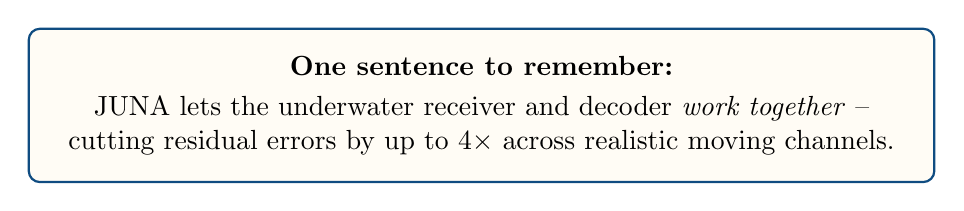
\begin{tikzpicture}
      \node[draw=accent,line width=0.8pt,rounded corners=4pt,fill=panel,
            minimum width=11.5cm,minimum height=1.7cm,inner sep=10pt,align=center,font=\normalsize] (s) {%
        \textbf{One sentence to remember:}\\[0.25em]
        JUNA lets the underwater receiver and decoder \emph{work together} \textendash{}\\
        cutting residual errors by up to $4\times$ across realistic moving channels.};
    \end{tikzpicture}
    \vspace{0.55cm}\par

    % decorative motion strip
    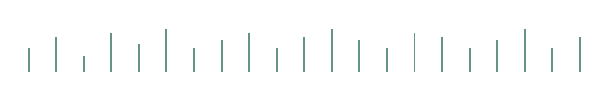
\begin{tikzpicture}[x=1cm,y=1cm]
      \foreach \x/\h in {0/0.30,0.35/0.45,0.70/0.20,1.05/0.50,1.40/0.35,1.75/0.55,2.10/0.30,2.45/0.40,2.80/0.50,3.15/0.30,3.50/0.45,3.85/0.55,4.20/0.40,4.55/0.30,4.90/0.50,5.25/0.45,5.60/0.30,5.95/0.40,6.30/0.55,6.65/0.30,7.00/0.45} {
        \draw[draw=juna!70,line width=0.7pt] (\x,0) -- (\x,\h);
      }
    \end{tikzpicture}

    \vspace{0.20cm}
    {\color{muted}\small Questions \textendash{} happy to go deeper on any slide.}
  \end{center}
\end{frame}

% =====================================================================
% BACKUP SLIDES (hidden, available if asked)
% =====================================================================
\appendix

\begin{frame}{Backup \textendash{} anticipated questions}
  \footnotesize
  \begin{columns}[T,onlytextwidth]
    \begin{column}{0.48\textwidth}
      \begin{beamercolorbox}[wd=\linewidth,sep=6pt,rounded=true]{calloutbox}
        \textbf{Q. ``Is this simulated or real?''}\\
        Results so far are simulations using \emph{physically modelled} shallow-water channels (range, depth, bottom type, surface state varied across 60 scenarios). Next step is replay testing with measured channels, then at-sea trials.
      \end{beamercolorbox}
      \vspace{0.3em}
      \begin{beamercolorbox}[wd=\linewidth,sep=6pt,rounded=true]{calloutbox}
        \textbf{Q. ``Hasn't someone solved this already?''}\\
        The conventional fix is more pilots or more complex equalisers. Both cost bandwidth or compute. JUNA reuses work the decoder already does, at modest extra cost.
      \end{beamercolorbox}
      \vspace{0.3em}
      \begin{beamercolorbox}[wd=\linewidth,sep=6pt,rounded=true]{calloutbox}
        \textbf{Q. ``Where does it not help?''}\\
        When carrier-to-carrier mixing is extreme (Channel E), the physics dominates and no receiver wins. JUNA never \emph{hurts}.
      \end{beamercolorbox}
    \end{column}
    \begin{column}{0.48\textwidth}
      \begin{beamercolorbox}[wd=\linewidth,sep=6pt,rounded=true]{calloutbox}
        \textbf{Q. ``What does the user see?''}\\
        Fewer dropped packets, fewer retransmissions, and \textendash{} where engineers want it \textendash{} higher useful data rate at the same reliability.
      \end{beamercolorbox}
      \vspace{0.3em}
      \begin{beamercolorbox}[wd=\linewidth,sep=6pt,rounded=true]{calloutbox}
        \textbf{Q. ``Will this fit on a real modem?''}\\
        Today's prototype is research-grade. A complexity-reduction pass is part of the next phase to bring it inside an embedded modem's budget.
      \end{beamercolorbox}
      \vspace{0.3em}
      \begin{beamercolorbox}[wd=\linewidth,sep=6pt,rounded=true]{calloutbox}
        \textbf{Q. ``How do we know when we've succeeded?''}\\
        Two yardsticks: (i) replay-channel BER matches simulation within tolerance; (ii) at-sea trial shows packet-error-rate reduction at fixed SNR and motion.
      \end{beamercolorbox}
    \end{column}
  \end{columns}
\end{frame}

\end{document}
